% SSEE — Paper 5: Israel-Stewart Causal Perturbative Analysis
% Compile: pdflatex (×2) + bibtex + pdflatex (×2)
\documentclass[12pt,a4paper]{article}

\usepackage[utf8]{inputenc}
\usepackage{amsmath,amssymb,amsfonts,amsthm}
\usepackage{graphicx}
\usepackage{booktabs}
\usepackage[colorlinks=true,linkcolor=red!70!black,citecolor=green!50!black,urlcolor=blue!80!black]{hyperref}
\usepackage{xcolor}
\usepackage{geometry}
\usepackage{natbib}
\usepackage{caption}
\usepackage{float}
\usepackage{array}
\usepackage{tabularx}
\usepackage{enumitem}
\usepackage{tcolorbox}
\usepackage{multirow}
\usepackage{mathtools}
\usepackage{physics}
\geometry{margin=2.5cm}
\emergencystretch=2em

% ── Custom commands ─────────────────────────────────────────────────────────
\newcommand{\SSEE}{\ifmmode\mathrm{SSEE}\else\textsc{ssee}\fi}
\newcommand{\LCDM}{\ifmmode\Lambda\mathrm{CDM}\else$\Lambda$CDM\fi}
\newcommand{\KALz}{\mathrm{KAL}_0}
\newcommand{\wz}{w_0}
\newcommand{\wa}{w_a}
\newcommand{\OmDE}{\Omega_{\mathrm{DE}}}
\newcommand{\Omm}{\Omega_{m}}
\newcommand{\cs}{c_{s}}
\newcommand{\tauPi}{\tau_\Pi}
\newcommand{\ztilde}{\tilde{\zeta}}
\newcommand{\Pitilde}{\tilde{\Pi}}
% \dd is already defined by the physics package
\newcommand{\Mpc}{\,\mathrm{Mpc}}
\newcommand{\kms}{\,\mathrm{km\,s^{-1}\,Mpc^{-1}}}

\graphicspath{{../results/figures/}}

% ── Title ───────────────────────────────────────────────────────────────────
\title{\textbf{Israel-Stewart Causal Viscous Perturbations\\
in the SSEE Dark Energy Framework:\\
Exact Marginal Stability, $\Lambda$CDM-Consistent Structure Growth,\\
and the Amplitude Ceiling}}

\author{Mike Edison Almeida Vallejo \\
\small \textit{Independent Researcher} \\
\small \href{mailto:mike.almeida1721@gmail.com}{mike.almeida1721@gmail.com} \\
\small ORCID: \href{https://orcid.org/0009-0008-2195-7836}{0009-0008-2195-7836}
}

\date{May 2026 \quad (SSEE, Paper~5 of~10)}

\sloppy
\begin{document}
\maketitle

% ── Abstract ────────────────────────────────────────────────────────────────
\begin{abstract}
The Structural Self-Energy Expansion (SSEE) derives a dark energy
equation of state $w_0 = -T_r/M_v \simeq -0.8399$ and $w_a \simeq -0.6700$
purely from the golden ratio $\varphi$ and $\pi$, with zero fitted
dimensionless parameters in the dark-energy background sector,
in agreement with the official DESI DR2 $w_0w_a$CDM posterior at $0.24\sigma$ (Pantheon+; $0.2$--$1.8\sigma$ across SN compilations).
(Following Paper~1 \S1.3, the broader SSEE programme carries a small set of
phenomenological ans\"atze in the dark-matter sector --- in particular the
$\phi$-DM mass and the non-minimal coupling $\xi$ --- retracted with the
$\varphi$-DM sector (Paper~6); OP-9/11 closed by dissolution, OP-14 resolved
in \texttt{OPEN\_PROBLEMS.md}; the present perturbation analysis is independent
of those ans\"atze.)
Because $w_0 < -1/3$, a naive $k$-essence interpretation gives a negative
bare sound speed $c^2_{s,\mathrm{bare}} = w_0 \simeq -0.840$, implying catastrophic
gradient instability on all sub-horizon scales.

We perform a linear Israel-Stewart (IS) causal viscous perturbation analysis of \SSEE\ dark energy in the sub-horizon regime,
addressing three interconnected questions:
\emph{(Q1)}~Does IS regularise the gradient instability for all observationally
relevant modes?
\emph{(Q2)}~Do linear IS perturbations dynamically source the CMB-to-dynamical
matter enhancement $\Omega_{m,\mathrm{CMB}}/\Omega_{m,\mathrm{dyn}}\approx2$, or
are the two matter sectors independent (the former interpretation as a
``$\mathrm{MIRA}$ factor'' having been retired in the $\omega_m$-direct reframe,
OP-8 dissolved)?
\emph{(Q3)}~What are the falsifiable predictions for the growth rate,
$\sigma_8$, and the $S_8$ parameter?

For Q1, we prove analytically that the SSEE structure constants satisfy the
algebraic identity $\ztilde/(\tauPi H_0) = |w_0|$, forcing
$c^2_{s,\mathrm{eff}}(k\to\infty) = 0$ to floating-point precision
(equivalently $\ztilde/(\tauPi H_0) = \OmDE$, since $\OmDE = |w_0|$ is the
saturation correspondence of Paper~1, Postulate~S, not an independent identity).
This is not a numerical coincidence but a construction-level identity:
any IS embedding of a dark-energy fluid satisfying
$\ztilde = |\wz|\,\tauPi H_0$ is exactly marginally stable, and the SSEE
structure constants admit such an embedding. We do not claim this as an
external theorem about all IS models, but as the consistency statement that
SSEE supports a stable IS extension at the construction level.
The critical wavenumber is $k_\mathrm{crit} = 0.456\,H_0/c$, placing the
instability boundary \emph{outside} the sub-horizon regime;
all modes with $k > H_0/c$ are causally stabilised. The margin
($k_\mathrm{crit}/H_0 c^{-1} \simeq 0.46$, a factor $\sim 2.2$ inside the
horizon) is comfortable at tree level. A future one-loop treatment would
test whether the stability regime is robust to QFT corrections; we
note this as an extension question rather than a current limitation.

For Q2, integrating the full linear IS perturbation ODE from $z=19$ to $z=0$
yields $\delta_{\mathrm{DE}}/\delta_m \to 0^-$ at all sub-horizon scales.
Consequently the numerical enhancement ratio is
$\Omega_{m,\mathrm{eff}}/\Omega_{m,\mathrm{dyn}} = 0.989\pm 0.017 \to 1$, not~$\approx2$:
linear IS perturbations do \emph{not} dynamically link the two matter sectors.
A background IS viscous calculation also fails to generate the factor (yielding
$\approx3.04$, not $\approx2$). The CMB-to-dynamical ratio $\approx1.93$ is therefore
not a fluid-dynamical effect.  Nor is it a ratio of two matter densities, as
earlier versions of this abstract stated: $\Omega_{m,\mathrm{dyn}}=0.160050$ is
not a density but $1+w_0$, a quantity of the equation of state, so the
difference $0.308881-0.160$ that once defined a second sector subtracts
objects of different kinds.  That construction is retracted (Paper~6).  The
matter content is a single sector, $\Omega_m = \omega_m/h^2 = 0.308881$, and
the algebraic number $\mathrm{MIRA}=(3\varphi+\pi)/4\simeq1.999$ survives only
as the Hubble-screening amplitude of Paper~9, no longer as a matter factor.

For Q3, we compute the IS growth index $\gamma_{\mathrm{IS}} = 0.5504 \pm 0.0003$
(consistent with $\gamma_{\Lambda\mathrm{CDM}} \simeq 0.55$), the growth
factor $\mathcal{G} = D_1^{\mathrm{SSEE}}/D_1^{\Lambda\mathrm{CDM}} = 1.0032$
(growth essentially identical to $\Lambda$CDM once the correct cosmological
background $\Omega_{m,\mathrm{cosm}} = 0.308881$ is used in the Poisson source;
see Paper~1, Sec.~1.4 (Two-$\Omega_m$ Criterion) for the rule that selects this
value over $\Omega_{m,\rm dyn}=0.160050$ on clustering scales),
and the predicted $S_8 = \sigma_8(\Omega_{m,\mathrm{CMB}}/0.3)^{0.5}$.
The amplitude is a separate matter and is not this paper's result.  Fixing
$A_s$ to Planck gives $S_8^{\mathrm{SSEE}} = 0.8256 \pm 0.0061$, and the
conservative CLASS ceiling is higher still, $S_8^{\mathrm{ceiling}} = 0.827$.
Both are \emph{ceilings under an imported normalisation}, not predictions:
$A_s$ is one of the two free CMB parameters of the model, and fixing it to
Planck imports the Planck--KiDS offset instead of predicting it.  With $A_s$
free and this same background, the fit to the raw KiDS-1000 $\xi_\pm$ gives
$S_8 = 0.7555\pm0.0192$, $0.11\sigma$ from KiDS-1000 (Paper~6).  What this
paper establishes is the growth \emph{shape}, $\mathcal{G}$ and
$\gamma_{\mathrm{IS}}$, which are amplitude-independent.
The $f\sigma_8$ mean tension is $0.70\sigma$, essentially identical to $\Lambda$CDM
($0.73\sigma$): SSEE does not suppress or enhance structure formation relative to
$\Lambda$CDM once $\Omega_{m,\mathrm{cosm}}=0.308881$ governs the growth equation.

Finally, we map the SSEE IS parameters to the EFT-of-dark-energy operator basis
\citep{Gubitosi2013,Bellini2015}, show that IS viscosity generates a unique
combination of the $\bar{M}_2^4$ braiding operator and a non-minimal kinetic
term, and demonstrate that the ghost condensate \citep{Arkani-Hamed2004}
and SSEE IS mechanisms are physically inequivalent: SSEE achieves \emph{exact}
marginal stability ($c^2_s=0$, the minimal-viscosity solution), while ghost condensation gives $c^2_s=1$.
\end{abstract}

\clearpage
{\small\tableofcontents}
\clearpage

%======================================================================
\section{Introduction}
\label{sec:intro}
%======================================================================

\subsection{The SSEE framework and the perturbation challenge}
\label{subsec:intro_ssee}

The Structural Self-Energy Expansion (SSEE) \citep{SSEE_Paper1} is a
minimal-parameter dark energy framework (zero fitted dimensionless parameters
in the background sector; see Paper~1 \S1.3) whose equation-of-state parameters
\begin{equation}
  w_0 = -\frac{T_r}{M_v}
  = -\frac{3(\varphi+\beta)}{\varphi+\pi+K_v}
  \simeq -0.8399, \qquad
  w_a = -\frac{P_{sc}}{I_g} \simeq -0.66997,
  \label{eq:w0_wa}
\end{equation}
are derived algebraically from the golden ratio $\varphi=(1+\sqrt{5})/2$ and $\pi$,
without any continuous free parameters.
Here $\beta=(\pi+\varphi)/2$, $K_v=\varphi+\pi+(\pi+\varphi)$,
$T_r=3(\varphi+\beta)$, $M_v=\varphi+\pi+K_v$, and $P_{sc}=(\pi+\varphi)+\varphi$.
The CPL parameters~\eqref{eq:w0_wa} \citep{ChevallierPolarski2001,Linder2003} are consistent with DESI DR2 at $0.24\sigma$ (Pantheon+)
\citep{SSEE_Paper2,AbdulKarim2025} and with Planck PR4 CMB spectra at
$\chi^2_r \leq 1.062$ \citep{SSEE_Paper3}.

Paper~4 \citep{SSEE_Paper4} identifies the algebraic structure constants
\begin{align}
  \KALz &\equiv \beta + \pi \simeq 5.5214
  \quad\text{(Structural Retention)}, \\
  \mathrm{MIRA} &\equiv \frac{3\varphi+\pi}{4} \simeq 1.9989
  \quad\text{(MIRA factor)},
\end{align}
and (under the $\omega_m$-direct reframe; OP-8 dissolved) the CMB matter
density is the standard physical $\Omega_{m,\mathrm{CMB}} = \omega_m/h^2
\simeq 0.308881$, built from the algebraic
$\omega_m=\omega_b+\omega_c+\omega_\nu$, in $0.88\sigma$ agreement with
Planck 2018. (The earlier MIRA mapping $\Omega_{m,\mathrm{dyn}}\times\mathrm{MIRA}\simeq0.3199$
is superseded.)

The present paper confronts a fundamental question that must be answered before
SSEE can claim theoretical consistency: \emph{does the dark energy sector remain
perturbatively stable}?

\subsection{The gradient instability problem}
\label{subsec:instability}

A canonical-kinetic (constant-$w$) $k$-essence proxy with Lagrangian $\mathcal{L} \propto X^n$
\citep{ArmendarizPicon2001},
where $X = -\tfrac{1}{2}\partial_\mu\phi\partial^\mu\phi$, has an adiabatic sound
speed $c^2_s = 1/(2n-1)$ and equation of state $w = 1/(2n-1)$, so $c^2_s = w$
\citep{Hu1998}.
For SSEE, $w_0 \simeq -0.840$, giving
\begin{equation}
  c^2_{s,\mathrm{bare}} = w_0 \simeq -0.840.
  \label{eq:cs2_bare}
\end{equation}
Negative $c^2_s$ signals a \emph{gradient instability}: perturbations
$\delta_{\mathrm{DE}} \propto e^{|c_s|kt}$ grow exponentially on a timescale
$(|c_s|k)^{-1}$, which for $k \gtrsim 10\,H_0/c$ (BAO scales) is shorter than a
Hubble time \citep{Caldwell2002}.
Left unchecked, this instability would generate excessive DE density contrast
$|\delta_{\mathrm{DE}}| \gg 1$, invalidating linear perturbation theory and
producing observable signatures in the CMB lensing and matter power spectra
inconsistent with data \citep{Calabrese2011}.

We stress that this bare instability is an artefact of the \emph{effective-fluid}
(constant-$w$) closure $c^2_s = w$, \emph{not} a property of the fundamental SSEE
field. The dark-energy action is the ghost condensate of Paper~7,
$K = c_1X + c_2X^2$ with $c_2X/c_1 = -0.522735$, which is independently
ghost-free and gradient-stable with adiabatic sound speed
\begin{equation}
  c^2_{s,\mathrm{ad}} = \frac{1+2u}{1+6u} = \frac{M_v-T_r}{5M_v+3T_r}
  = 0.021284 ,
  \qquad u \equiv c_2X/c_1 ,
\end{equation}
a clustered rather than smooth dark energy.
%
\emph{Correction (2026-09-06).} Earlier versions of this paragraph quoted
$c^2_{s,\mathrm{ad}}\in[0.60,1]$ and attributed the Lagrangian to ``Papers~7
and~10''. That value was computed from $K(X)=X/\KALz+X^2/M^4$, which is
Paper~10's \emph{screening} functional and not the dark-energy action: the two
carry different coefficient ratios ($+0.008577$ against $-0.522735$) and do
different jobs \citep{SSEE_Paper10}. The sound speed of the dark-energy sector
is the one above.
The IS analysis below addresses the \emph{hydrodynamic} (fluid) description used
by Boltzmann codes, where dark energy is parametrised by $(w, c^2_s)$ and the
naive closure $c^2_s = w$ would be catastrophic.
The IS bulk viscosity is $\ztilde = \KALz/3$, so the fluid-level regularisation
introduces no new parameter.

\emph{What is and is not fixed here (2026-09-07).} Only the \emph{ratio}
enters the observable: $\ztilde/(\tauPi H_0) = \OmDE$, and since $\ztilde$ and
$\tauPi$ share the factor $\KALz$, it cancels. The marginal-stability result
$c^2_{s,\rm eff} = \wz + \OmDE = 0$ is therefore \emph{independent of}
$\KALz$: replacing it by any positive constant returns the same $0$, which
follows from the algebraic identity $\OmDE = |\wz|$ alone. The individual split
$\ztilde = \KALz/3$ is consequently not determined by anything in \emph{this}
observable, and is not claimed to be.

It does not follow that the IS constants are unconstrained. $\KALz$ enters the
framework in three places that do move observables: $\omega_c =
\KALz\,\omega_b\,n_s$ (a $10\%$ shift moves $\omega_c$ by $\sim\!10\sigma$
against Planck); the neutrino sum $\Sigma m_\nu = R_2\,\omega_b\,(93.14)/(\tauPi
H_0)$, where $\KALz$ appears \emph{squared} through $R_2 = \Omega/(\KALz T_r)$
and $\tauPi H_0 = \KALz/(3\OmDE)$, so that $\KALz \to 1.1\,\KALz$ gives
$\Sigma m_\nu = 0.0566$~eV, \emph{below} the oscillation floor $0.058$~eV and
therefore falsified; and Paper~10's screening functional. The cancellation
above is thus local to $c^2_{s,\rm eff}$: $\tauPi$ itself is anchored, through
$\Sigma m_\nu$, to within roughly $10\%$.

\emph{Correction (2026-09-07).} Earlier versions of this passage read
``the same structural constant $\KALz$ that normalises $K(X)$ also fixes the IS
bulk viscosity''. That is wrong about \emph{which} $K(X)$: $\KALz$ does not
appear in the dark-energy action at all --- Paper~7's kinetic function is
$K = c_1X + c_2X^2$, and the $X/\KALz$ form belongs to Paper~10's screening
functional. Worse, the dark-energy action \emph{cannot} supply a bulk
viscosity: for shift-symmetric $K(X)$ the pressure perturbation is exactly
adiabatic, $\delta p - c^2_s\,\delta\rho = 0$ identically in $(c_1,c_2,X)$, so
the entropy production of Eq.~\eqref{eq:entropy_prod} vanishes and $\zeta = 0$.
The IS layer is therefore a repair of the $(w,c^2_s)$ \emph{parametrisation}
imposed by Boltzmann codes, not a property of the field; the sector's own
prediction is the field value $c^2_s = 0.021284$. The recurrence of $\KALz$ in
$\ztilde$ is a resemblance across two different objects, not a derivation of one
from the other, and is not claimed as one. See \textbf{OP-22b}.

\subsection{The Israel-Stewart resolution}
\label{subsec:IS_intro}

The first-order (Eckart) relativistic fluid theory \citep{Eckart1940} is acausal
\citep{Muller1967} and generically unstable \citep{HiscockLindblom1985}: perturbations propagate at
infinite speed.
Israel \citep{Israel1976} and Israel \& Stewart \citep{IsraelStewart1979}
constructed a second-order causal theory in which dissipative fluxes satisfy
relaxation equations with a finite relaxation time $\tauPi$.
Perturbations then propagate causally (speed $\leq c$), and the theory is
thermodynamically stable provided $\tauPi > 0$ and the bulk viscosity $\zeta \geq 0$
\citep{HiscockLindblom1983}.
The modern form of IS equations has been derived systematically from the Boltzmann
equation \citep{Denicol2012}, confirming the causal structure at second order.
Bulk-viscous cosmological models have been explored phenomenologically in
\citet{Brevik2005}, motivating the present IS dark-energy application.

SSEE identifies in Paper~1 a structural IS steady-state condition that fixes
$\KALz$ as the dimensionless viscosity, implying specific values of both $\zeta$
and $\tauPi$ with no additional freedom.
The central claim of the present paper is that \emph{these algebraically determined
IS parameters exactly neutralise the gradient instability}.

\subsection{Paper structure}
\label{subsec:outline}

Section~\ref{sec:theory} derives the IS perturbation equations from the entropy
current divergence, establishes thermodynamic consistency, and introduces
the quasi-static approximation.
Section~\ref{sec:Q1_stability} establishes the marginal stability identity (under minimality) and
characterises the critical wavenumber.
Section~\ref{sec:Q2_MIRA} presents numerical integration results for the MIRA test.
Section~\ref{sec:growth} derives the growth index, $\sigma_8$, and $S_8$
prediction, addressing the weak-lensing tension.
Section~\ref{sec:EFT} maps the IS mechanism to the EFT-of-dark-energy operator basis.
Section~\ref{sec:discussion} discusses physical implications, and
Section~\ref{sec:conclusions} states the falsifiable predictions.
Appendices contain the full IS dispersion relation derivation (Appendix~\ref{app:dispersion}),
eigenvalue analysis of the perturbation matrix (Appendix~\ref{app:eigenvalues}),
and the background IS Friedmann modification.

%======================================================================
\section{Israel-Stewart Theory for SSEE Dark Energy}
\label{sec:theory}
%======================================================================

\subsection{Entropy production and the second-order IS equations}
\label{subsec:entropy}

In relativistic thermodynamics the second law requires
$\nabla_\mu S^\mu \geq 0$, where $S^\mu = su^\mu - q^\mu/T + \cdots$
is the entropy 4-current \citep{Weinberg1971,Israel1976,IsraelStewart1979}.
For a cosmological fluid with only bulk viscosity, the divergence of the entropy
current to second order in deviations from equilibrium is
\begin{equation}
  \nabla_\mu S^\mu = \frac{1}{T}\!\left[-\Pi\,\theta
    - \frac{\tauPi}{2\zeta T}\,\Pi\,\dot{\Pi}
    - \frac{\Pi^2}{\zeta}\right] \geq 0,
  \label{eq:entropy_prod}
\end{equation}
where $\theta = \nabla_\mu u^\mu = 3H$ is the expansion scalar,
$\Pi$ is the bulk viscous pressure (beyond the thermodynamic pressure $p$),
$\zeta \geq 0$ is the bulk viscosity coefficient, and
$\tauPi \geq 0$ is the relaxation time.
Minimising the quadratic form subject to $\nabla_\mu S^\mu \geq 0$ yields the
Israel-Stewart bulk viscous relaxation equation
\begin{equation}
  \tauPi\,\dot{\Pi} + \Pi = -3\zeta H
    - \frac{\tauPi\,\Pi}{2}\left[\frac{\dot{\tauPi}}{\tauPi}
    - \frac{\dot{\zeta}}{\zeta} - \frac{\dot{T}}{T}\right],
  \label{eq:IS_full}
\end{equation}
which reduces in the cosmologically relevant slow-variation limit
($|\dot{\tauPi}/\tauPi|, |\dot{\zeta}/\zeta| \ll H$) to
\begin{equation}
  \boxed{\tauPi\,\dot{\Pi} + \Pi = -3\zeta H.}
  \label{eq:IS_simple}
\end{equation}
This is the form used throughout this paper.
Two properties follow immediately from Eq.~\eqref{eq:entropy_prod}:
\begin{enumerate}
  \item \textbf{Causality}: the IS relaxation limits signal propagation to
    $v_{\rm sig} = \sqrt{\zeta/[\tauPi(\rho_{\mathrm{DE}}+p_{\mathrm{DE}})]} < c$
    \citep{HiscockLindblom1983} --- the enthalpy again, as the inertia of the
    propagating mode.
  \item \textbf{Stability}: the entropy production rate is non-negative for all
    $\Pi$ provided $\tauPi > 0$ and $\zeta \geq 0$.
\end{enumerate}
Both conditions are satisfied in SSEE (established in Section~\ref{sec:Q1_stability}).

\subsection{SSEE IS parameters from algebraic structure constants}
\label{subsec:IS_params}

In the SSEE steady state $\dot{\Pi}=0$, Eq.~\eqref{eq:IS_simple} gives
$\Pi = -3\zeta H$.
The dimensionless viscosity and relaxation time are defined by normalising to
the dark-energy \emph{enthalpy} and the Hubble rate:
\begin{align}
  \ztilde &\equiv \frac{\zeta}{(\rho_{\mathrm{DE}}+p_{\mathrm{DE}})\,H_0}
           = \frac{\zeta}{\rho_{\mathrm{DE}}(1+\wz)\,H_0}, \\
  \tauPi H_0 &\equiv \text{dimensionless IS relaxation time}.
\end{align}
The enthalpy $\rho+p$, not the density $\rho$, is the correct normalisation:
it is the inertia that appears in the relativistic Euler equation
(Appendix~\ref{app:dispersion}, second line) and the origin of the $1/(1+w)$
factor multiplying the pressure gradient in the standard fluid perturbation
equations. Normalising this way makes $\ztilde/(\tauPi H_0)$ directly a squared
sound speed, with no residual factors.

\begin{tcolorbox}[colback=green!4,colframe=green!45!black,
  title={\textbf{Resolved: the normalisation of $\ztilde$ (OP-22, closed 2026-09-06)}}]
A previous version of this box reported $c^2_{s,\mathrm{eff}}=0$ as an artefact
of a normalisation mismatch between documents. That diagnosis was wrong, and we
correct it here rather than leave it standing.

\emph{The question.} $\ztilde=\KALz/3$ is a dimensionless viscosity, but
dimensionless \emph{with respect to what}? The candidates differ by large
factors, because one physical quantity $\zeta/(\rho\,\tauPi)$ takes three values
depending on the divisor:
\begin{center}
\begin{tabular}{lc}
\toprule
divisor & $\zeta/(\rho\,\tauPi)$ \\
\midrule
$\rho_{\rm crit}$ (total)         & $0.839950$ \\
$\rho_{\rm DE}$                   & $1.000000$ \\
$\rho_{\rm DE}+p_{\rm DE}$ (enthalpy) & $6.248039$ \\
\bottomrule
\end{tabular}
\end{center}

\emph{The evidence, and it is not unanimous.} Three places in the framework fix
the normalisation, and one of them points the other way. The steady-state
ansatz as originally written, $\Pi = -\KALz\,\rho_{\rm DE}H$, gives
$\zeta = \KALz\rho_{\rm DE}/3$ and hence
$c^2_{s,\mathrm{eff}} = \wz + 5.248 = +4.41$: superluminal, and therefore not
an option. The two operative appendices of this paper both require the other
convention.

\emph{The answer, from two independent witnesses inside this paper.}
The relativistic inertia of a sound wave is the enthalpy, so the dispersion
relation of Appendix~\ref{app:dispersion} carries
$\zeta/[\tauPi(\bar\rho+\bar p)]$; it reduces to $\ztilde/(\tauPi H_0)$
\emph{only if} $\ztilde$ is enthalpy-normalised, $\zeta =
\ztilde\,(\rho_{\rm DE}+p_{\rm DE})H_0$, which is what that appendix states.
Independently, the eigenvalue analysis of Appendix~\ref{app:eigenvalues} uses
$\mathcal{F}=(1-3c^2_s)+\ztilde(k/H)^2 \approx 186$ at $k=10$: the
enthalpy normalisation returns $185.05$, whereas normalising to $\rho_{\rm crit}$
returns $1370$, an order of magnitude off. Both appendices therefore use the
same convention, and it is the enthalpy one.

\emph{The resolution, and why it is not merely a choice.} We adopt the
enthalpy form of the steady-state condition,
$\Pi = -\KALz\,(\bar\rho+\bar p)\,H$. The decisive argument is a limit test,
independent of anything in SSEE. Take $w \to -1$ exactly. Then
$\bar\rho+\bar p \to 0$: a cosmological constant carries no fluid degrees of
freedom, so its bulk viscous pressure \emph{must} vanish. The enthalpy form
gives $\Pi \to 0$ automatically; the $\rho_{\rm DE}$ form gives a finite
viscous pressure for a cosmological constant, which is not a viable
hydrodynamic limit. Two further reasons agree: it is what both appendices of
this paper already use, and it is the form consistent with relativistic
dissipative hydrodynamics, where the enthalpy is the inertia in the Euler
equation and in the bulk-viscous transport alike
\citep{Maartens1996,HiscockLindblom1985}. That the alternative is superluminal
is then a consequence, not the reason for choosing. The archived note in which
the $\rho_{\rm DE}$ form was first written is superseded by this.

\emph{Consequence.} $c^2_{s,\mathrm{eff}} = \wz + \ztilde/(\tauPi H_0)
= \wz + \OmDE = 0$ stands: marginally stable, manifestly subluminal, and
\textbf{not} an artefact. The $0$ is a result.

\emph{What \emph{is} withdrawn.} The \emph{justification} of $\tauPi$ given in
the EFT appendix of Paper~1 \citep{SSEE_Paper1}, which claimed to derive
$\tauPi H_0 = \KALz/(3\OmDE)$ by saturating the causality bound written as
$\zeta/(\rho_{\rm DE}\tauPi)\le 1$. That bound uses $\rho$ where the enthalpy
belongs; imposed correctly it returns $\tauPi H_0 = \ztilde(1+\wz) = 0.2946$,
not $2.191$. The factor between them is exactly $(1+\wz)^{-1}=6.248$. Nothing
numerical moves --- $\tauPi H_0 = \KALz\Omega/T_r$ is algebra, and was already
stated in that form in Eq.~\eqref{eq:IS_params} --- but causality does not
\emph{derive} it, and Paper~1 no longer claims that it does.

\emph{Residual, still open --- and smaller than it looked.} The framework
carries two sound speeds for the dark-energy sector:
\begin{center}
\begin{tabular}{lcc}
\toprule
mode & source & $c^2_s$ \\
\midrule
viscous fluid (this paper) & IS, $\wz+\OmDE$ & $0$ \\
field, adiabatic & Paper~7 ghost condensate & $0.021284$ \\
\bottomrule
\end{tabular}
\end{center}
They are not in conflict in character --- both describe a \emph{clustered}
dark energy, $c^2_s \ll 1$. \emph{Update (2026-09-07): they are not two
channels.} A $k$-essence scalar carries exactly one propagating scalar degree
of freedom (Paper~7, kinetic matrix $K_X+2XK_{XX}$), and in the IS fluid the
bulk viscous pressure $\Pi$ is a relaxing auxiliary slaved to the density
perturbation, not a second propagating mode. Both descriptions therefore
count \emph{one} mode, so the two numbers are two descriptions of the same
wave and the field one is the fundamental of the pair: it comes from the
action. The fluid description additionally borrows $c^2_{s,\rm ad}=\wz<0$,
which is gradient-unstable on its own and is precisely what the viscosity
rescues to $0$; the field needs no such rescue, returning $+0.021284$
directly. What remains open, and is now the whole of \textbf{OP-22b}, is
narrower: the map from the field parameters to the effective fluid
$(\ztilde,\tauPi)$ is not derived, so \emph{why} the fluid limit lands
exactly on $0$ rather than on $0.021284$ is not established. The gap is the
whole of Paper~7's prediction, so a measurement of $c^2_s$ remains sharp.
\end{tcolorbox}

\noindent With the steady-state condition as currently written, and combined
with the IS equation, one obtains \citep{SSEE_Paper1}:
\begin{equation}
  \boxed{\ztilde = \frac{\KALz\,\Omega}{M_v} = \frac{\KALz}{3} \simeq 1.8405,
  \qquad
  \tauPi H_0 = \frac{\KALz\,\Omega}{T_r} \simeq 2.191.}
  \label{eq:IS_params}
\end{equation}
Written this way the two are manifestly the \emph{same} construction, built
from the same parents $(\KALz,\Omega)$ and differing only in which sovereignty
sits in the denominator: $T_r$ (TRIAL) for the relaxation time, $M_v$ (ATLAS)
for the viscosity. The factor $3$ in $\KALz/3$, which looks arbitrary in
isolation, is simply $M_v = 3\Omega$. Both parameters are determined solely by
$\KALz = \beta+\pi$, $\Omega=\varphi+\pi$ and the sovereignties — no freedom
remains.
The ratio
\begin{equation}
  \frac{\ztilde}{\tauPi H_0} = \frac{\KALz/3}{\KALz/(3\OmDE)} = \OmDE = |\wz|
  \label{eq:ratio_identity}
\end{equation}
is an exact algebraic identity in SSEE; its stability consequence is derived
in Section~\ref{sec:Q1_stability}.

\subsection{Thermodynamic consistency}
\label{subsec:thermodynamic}

The IS theory is thermodynamically consistent if and only if:
\begin{enumerate}[label=(\roman*)]
  \item $\tauPi > 0$: satisfied, $\tauPi H_0 = 2.191 > 0$.
  \item $\zeta \geq 0$: satisfied, $\ztilde = 1.841 > 0$.
  \item The signal speed $v_{\rm sig} = \sqrt{\zeta/(\tauPi\rho_{\mathrm{DE}})}
    = \sqrt{\ztilde/(\tauPi H_0)/\OmDE}$:\\
    in SSEE: $v_{\rm sig}/c = \sqrt{|\wz|/\OmDE} = \sqrt{1} = 1$,
    so $v_{\rm sig} = c$ exactly. The signal speed saturates the causality bound.
\end{enumerate}
The fact that $v_{\rm sig} = c$ is another algebraic consequence of
Eq.~\eqref{eq:ratio_identity}: $\ztilde/(\tauPi H_0) = \OmDE = |\wz|$, and
$v_{\rm sig}^2/c^2 = \ztilde/((\tauPi H_0)\OmDE) = 1$.
This means SSEE dark energy perturbations propagate exactly at the speed of light
in the IS high-$k$ limit — the maximally causal configuration consistent with
thermodynamic stability.

\subsection{Linearised perturbation equations in Newtonian gauge}
\label{subsec:perturb_eqs}

In Newtonian gauge ($\Phi$ = gravitational potential) with $d/d\ln a$ derivatives
(prime notation), the linearised continuity, Euler, and IS relaxation equations
for a two-fluid system (pressureless CDM + IS dark energy) in the sub-horizon
limit $k \gg aH$ are \citep{Hu1998,Maartens1996}:
\begin{align}
  \delta'_m &= -\frac{k}{aH}\,v_m + 3\Phi',
  \label{eq:deltam} \\
  v'_m      &= -v_m - \frac{k}{aH}\,\Phi,
  \label{eq:vm} \\
  \delta'_{\mathrm{DE}} &= -(1+w)\!\left[\frac{k}{aH}\,v_{\mathrm{DE}} - 3\Phi'\right],
  \label{eq:deltaDE} \\
  v'_{\mathrm{DE}} &= -(1-3c^2_s)\,v_{\mathrm{DE}}
    - \frac{k}{aH}\!\left[\frac{c^2_s\,\delta_{\mathrm{DE}}}{1+w}
    + \frac{\Phi}{1+w} - \Pitilde\right],
  \label{eq:vDE} \\
  \tauPi H\,\Pitilde' &= -\Pitilde - \ztilde\,\frac{k}{aH}\,v_{\mathrm{DE}},
  \label{eq:Pi}
\end{align}
where $w = \wz + \wa(1-a)$ is the CPL equation of state,
$\Pitilde$ is the dimensionless bulk viscous pressure perturbation normalised
to $\rho_{\mathrm{DE}}$, and the Newtonian potential satisfies
\begin{equation}
  \frac{k^2}{a^2}\Phi = -\frac{3H_0^2}{2a}\!\left[\Omega_m(a)\,\delta_m
    + \OmDE\,f_{\mathrm{DE}}(a)\,\delta_{\mathrm{DE}}\right],
  \label{eq:Poisson}
\end{equation}
with $f_{\mathrm{DE}}(a) = \rho_{\mathrm{DE}}(a)/\rho_{\mathrm{DE},0}$.
The $3\Phi'$ terms in Eqs.~\eqref{eq:deltam}--\eqref{eq:deltaDE} arise from the
metric perturbation and are retained for completeness; in the deep sub-horizon
limit $k \gg aH$ they are subdominant and we drop them in the numerical integration,
consistent with standard practice \citep{Hu1998}.

\subsection{Quasi-static IS approximation and stiffness reduction}
\label{subsec:QS}

The IS relaxation eigenvalue is $\lambda_\Pi \approx -(\tauPi H)^{-1}$.
At $z=0$, $\tauPi H = \tauPi H_0 \cdot (H/H_0) = 2.191$;
at $z=99$, $H/H_0 \approx 400$, so $\tauPi H \approx 876$.
The Eq.~\eqref{eq:Pi} ODE is therefore stiff: the $\Pitilde$ mode relaxes
on a timescale $\sim 1/(876 H)$ at early times, orders of magnitude faster
than the growing mode.

Setting $\Pitilde' = 0$ in Eq.~\eqref{eq:Pi} (quasi-static IS approximation,
valid when $\tauPi H \gg 1$) yields the algebraic relation
\begin{equation}
  \Pitilde_{\mathrm{QS}} = -\ztilde\,\frac{k}{aH}\,v_{\mathrm{DE}},
  \label{eq:PiQS}
\end{equation}
which substituted into Eq.~\eqref{eq:vDE} gives an effective velocity friction:
\begin{equation}
  v'_{\mathrm{DE}} = -\underbrace{\!\left[(1-3c^2_s)
    + \ztilde\!\left(\frac{k}{aH}\right)^{\!2}\right]}_{\mathcal{F}(k,a)}\!
    v_{\mathrm{DE}}
    - \frac{k}{aH}\,\frac{c^2_s\,\delta_{\mathrm{DE}}}{1+w}
    - \frac{k}{aH}\,\frac{\Phi}{1+w}.
  \label{eq:vDE_QS}
\end{equation}
The effective friction $\mathcal{F} = (1-3c^2_s) + \ztilde(k/aH)^2$ is dominated
at large $k$ by the viscous term $\ztilde(k/aH)^2 \propto k^2$, which grows without
bound.
This $k^2$ suppression is the physical mechanism behind IS stabilisation of
DE perturbations.
The 5-variable stiff ODE system
(Eqs.~\ref{eq:deltam}--\ref{eq:Pi}) is thus reduced to a 4-variable system
($\delta_m, v_m, \delta_{\mathrm{DE}}, v_{\mathrm{DE}}$) integrable with
standard Runge-Kutta methods.

\begin{table}[h!]
\centering
\caption{Background cosmology and IS relaxation parameters across cosmic history.
  $H/H_0$ is computed from the SSEE CPL Friedmann equation with the matter
  density $\Omega_m=0.308881$ and CPL dark energy.%
% 2026-09-07: esta tabla se calculaba con Omega_m,dyn = 0.160050 en la ranura
% de DENSIDAD de la ecuacion de Friedmann. Ese numero es 1+w_0, la ecuacion de
% estado, y entra por la presion, nunca como densidad de materia (Paper 1
% Sec. two_omega_m, donde el criterio de dos Omega_m se declara retirado; y es
% el mismo bug que inflaba chi2_BAO a 726 antes del fix de geometria del
% 2026-07-09). Recalculada con Omega_m = 0.308881: H/H_0 sube hasta un 38.9%
% a alto z (400.1 -> 555.8 en z=99; 1.441 -> 1.768 en z=1; sin cambio en z=0,
% donde E=1 por definicion), y tau_Pi H sube en la misma proporcion. La
% CONCLUSION de la tabla no cambia: los valores corregidos son MAYORES, o sea
% que la aproximacion cuasi-estatica es aun mejor de lo que se publicaba. Las
% etiquetas de validez se conservan.
  $\tauPi H$ shows that the quasi-static approximation ($\tauPi H \gg 1$) is
  excellent at all redshifts.}
\label{tab:background}
\begin{tabular}{ccccc}
\toprule
$z$ & $a$ & $H/H_0$ & $\tauPi H$ & QS validity \\
\midrule
99   & 0.010 & 555.8 & 1218   & $\gg 1$ \\
19   & 0.050 & 49.71 & 108.9  & excellent \\
9    & 0.100 & 17.58 & 38.52  & excellent \\
4    & 0.200 & 6.237 & 13.67  & very good \\
1    & 0.500 & 1.768 & 3.873  & adequate \\
0.25 & 0.800 & 1.157 & 2.534  & marginal \\
0    & 1.000 & 1.000 & 2.191  & marginal \\
\bottomrule
\end{tabular}
\end{table}

\paragraph{QS error estimate.}
At $z=0$, $\tauPi H = 2.191$, so the adiabatic correction to the
quasi-static approximation is of order $(\tauPi H)^{-1} \simeq 0.46$.
However, this error in $\Pi$ propagates to matter growth through a
two-step coupling: $\Delta\Pi \to \Delta v_{\mathrm{DE}} \to
\Delta\delta_{\mathrm{DE}} \to \Delta\Phi \to \Delta\delta_m$.
At sub-Hubble scales, the IS effective friction in the DE Euler equation
is $\mathcal{F} \approx \ztilde(k/aH)^2$; for $k \geq 5\,H_0/c$ this
gives $\mathcal{F} \geq 46$, so the fractional error in $v_{\mathrm{DE}}$
is $\lesssim 0.46/46 \approx 1\%$.
The resulting error in the growth factor $D_1$ is further suppressed by
$\Omega_{\mathrm{DE}}\,\delta_{\mathrm{DE}}/(\Omega_m\,\delta_m) \lesssim
5\%$ at $k \geq 5\,H_0/c$, giving $\Delta D_1/D_1 \lesssim 0.05\%$ for
the BAO scales that dominate the $\sigma_8$ integral.
Only super-Hubble modes ($k \sim H_0/c$) carry an $\mathcal{O}(25\%)$
DE-sector error, but these modes contribute negligibly to $\sigma_8$
(filtered by $W(8\,\mathrm{Mpc}/h)$).
The QS approximation therefore introduces a sub-percent bias on all
reported $\sigma_8$, $S_8$, and $f\sigma_8$ values.

%======================================================================
\section{Q1: Gradient Stability — Exact Marginal Stability Theorem}
\label{sec:Q1_stability}
%======================================================================

\subsection{IS dispersion relation from linear perturbation theory}
\label{subsec:dispersion}

For a relativistic viscous fluid with IS relaxation, the full dispersion relation
for DE perturbations is (derived in Appendix~\ref{app:dispersion}):
\begin{equation}
  \omega^2 = c^2_{s,\mathrm{bare}}\,k^2
    + i\omega\,\frac{\zeta\,k^2}{\rho_{\mathrm{DE}}\,(\tauPi\omega + i)}
    - \frac{k^2}{a^2}\,\frac{3H^2\OmDE}{k^2/a^2}.
  \label{eq:disprel_full}
\end{equation}
In the short-wavelength limit $k\tauPi \gg aH$ (IS regime,
$|\omega|\tauPi \gg 1$), the damping term saturates and the dispersion relation
simplifies to
\begin{equation}
  \omega^2 = \left(c^2_{s,\mathrm{bare}} + \frac{\ztilde}{\tauPi H_0}\right)k^2
  \equiv c^2_{s,\mathrm{eff}}\,k^2.
  \label{eq:cs2_eff_def}
\end{equation}
The full $k$-dependent interpolation between the Navier-Stokes ($k\to 0$) and
IS ($k\to\infty$) limits is
\begin{equation}
  c^2_{s,\mathrm{eff}}(k) = c^2_{s,\mathrm{bare}}
  + \frac{\ztilde}{\tauPi H_0}\cdot\frac{x^2}{1+x^2},
  \quad x \equiv \frac{k\,c\,\tauPi H_0}{aH},
  \label{eq:cs2full}
\end{equation}
where $x$ is the dimensionless IS parameter measuring the ratio of the mode
wavenumber to the IS relaxation scale.

\subsection{Marginal stability under minimality}
\label{subsec:identity}

\begin{tcolorbox}[colback=blue!5!white,colframe=blue!60!black,title={\textbf{SSEE Marginal Stability (given minimality)}}]
\textit{In the SSEE dark energy framework, the IS parameters satisfy}
\begin{equation}
  \frac{\ztilde}{\tauPi H_0}
  = \frac{\KALz/3}{\KALz/(3\,\OmDE)}
  = \OmDE = |\wz|,
\end{equation}
\textit{and therefore}
\begin{equation}
  c^2_{s,\mathrm{eff}}(k\to\infty)
    = c^2_{s,\mathrm{bare}} + |\wz|
    = \wz + |\wz| = 0.
\end{equation}
\textit{This is an exact algebraic identity within the SSEE constants, not a
numerical coincidence. It expresses a construction-level consistency rather
than a theorem constraining all IS models: SSEE supports an IS embedding for
which dark-energy perturbations are exactly marginally stable in the
high-$k$ limit.}
\end{tcolorbox}

\vspace{6pt}
The proof follows directly from Eq.~\eqref{eq:ratio_identity}.
The numerical verification gives $|c^2_{s,\mathrm{eff}}| = 3.1\times 10^{-16}$
(floating-point round-off, confirming machine-precision exactness).

The physical significance is the following:
\begin{itemize}
  \item The gradient instability present for $k < k_\mathrm{crit}$
    (Navier-Stokes regime) is completely neutralised for $k > k_\mathrm{crit}$
    (IS regime).
  \item The neutralisation is \emph{exact}: $c^2_{s,\mathrm{eff}} = 0$ means
    DE perturbations propagate as effectively pressureless dust at small scales,
    exactly as required for consistency with CMB and LSS observations.
  \item The result holds at all redshifts since $\ztilde$ and $\tauPi$ are
    background-level constants in SSEE.
\end{itemize}

\subsection{Uniqueness of the minimal-viscosity solution}
\label{subsec:uniqueness}

The condition $c^2_{s,\mathrm{eff}} = 0$ requires $\ztilde/(\tauPi H_0) = |c^2_{s,\mathrm{bare}}|$.
For a general dark fluid with $w_0 < 0$, this is a \emph{fine-tuning} condition
relating the viscosity to the equation of state.
In SSEE both sides equal $\OmDE = |\wz|$, and the $\KALz$ dependence cancels
in the ratio $\ztilde/(\tauPi H_0) = (\KALz\Omega/M_v)/(\KALz\Omega/T_r) = T_r/M_v$.
No number is tuned.

We are explicit about what does the work, because it is easy to overclaim here.
The relaxation time $\tauPi H_0 = \KALz\Omega/T_r$ is fixed independently in
Paper~1 \citep{SSEE_Paper1}, and $\wz = -T_r/M_v$ is fixed independently in the
background sector. Given those two, requiring $c^2_{s,\mathrm{eff}}=0$ leaves
\emph{no} freedom in $\ztilde$: it must equal $|\wz|\,\tauPi H_0
= \KALz\Omega/M_v$, with the $T_r$ cancelling identically. So $\ztilde$ is not
an independent input.

What remains an input is the \emph{requirement} of marginal stability itself,
and it is a selection principle rather than a fitted number. Its justification
is minimality: since $c^2_{s,\mathrm{bare}} = \wz < 0$ is a gradient
instability, some viscosity is mandatory, and $\ztilde = \KALz\Omega/M_v$ is
the \emph{smallest} value that removes it --- any less leaves the instability,
any more is unmotivated surplus. We therefore state the result as a consequence
of minimality, not as a prediction free of assumptions.

\subsection{Critical wavenumber and observational window}
\label{subsec:kcrit}

The IS stabilisation transition occurs at $x = 1$, defining the critical wavenumber
\begin{equation}
  k_\mathrm{crit}(a) = \frac{aH}{c\,\tauPi H_0}.
\end{equation}
At $z=0$ ($a=1$, $H=H_0$):
\begin{equation}
  \frac{k_\mathrm{crit}}{H_0/c}
  = \frac{1}{\tauPi H_0}
  = \frac{1}{2.191}
  \simeq 0.456.
  \label{eq:kcrit_z0}
\end{equation}
Note: this differs from the expression $1/(\tauPi H_0 |c_s|)$ used in
Section~\ref{sec:intro} because the $|c_s|$ factor enters the dispersion
relation at the Navier-Stokes level; the IS transition properly occurs at $x=1$.
Since $k_\mathrm{crit} \simeq 0.456\,H_0/c < H_0/c$, the critical scale
lies \emph{below} the Hubble wavenumber.
Every sub-horizon mode satisfies $k > aH/c = H_0/c$ at $z=0$,
i.e.\ $k > k_\mathrm{crit}$: all sub-horizon modes are IS-stabilised.

At higher redshift $k_\mathrm{crit}(z) = k_\mathrm{crit}(0) \times H(z)/H_0$,
which grows with redshift.
However, for a given comoving mode $k$, it entered the IS-stable regime at
$a_\mathrm{stab}(k) = k\,c\,\tauPi H_0/H(a_\mathrm{stab})$.
For BAO scales ($k \approx 0.1\,\mathrm{Mpc}^{-1} \approx 230\,H_0/c$),
$a_\mathrm{stab} \ll 10^{-3}$: these modes were IS-stable well before matter-radiation
equality.
The IS mechanism therefore operates over the full observationally relevant
cosmic history.

\begin{figure}[h!]
\centering
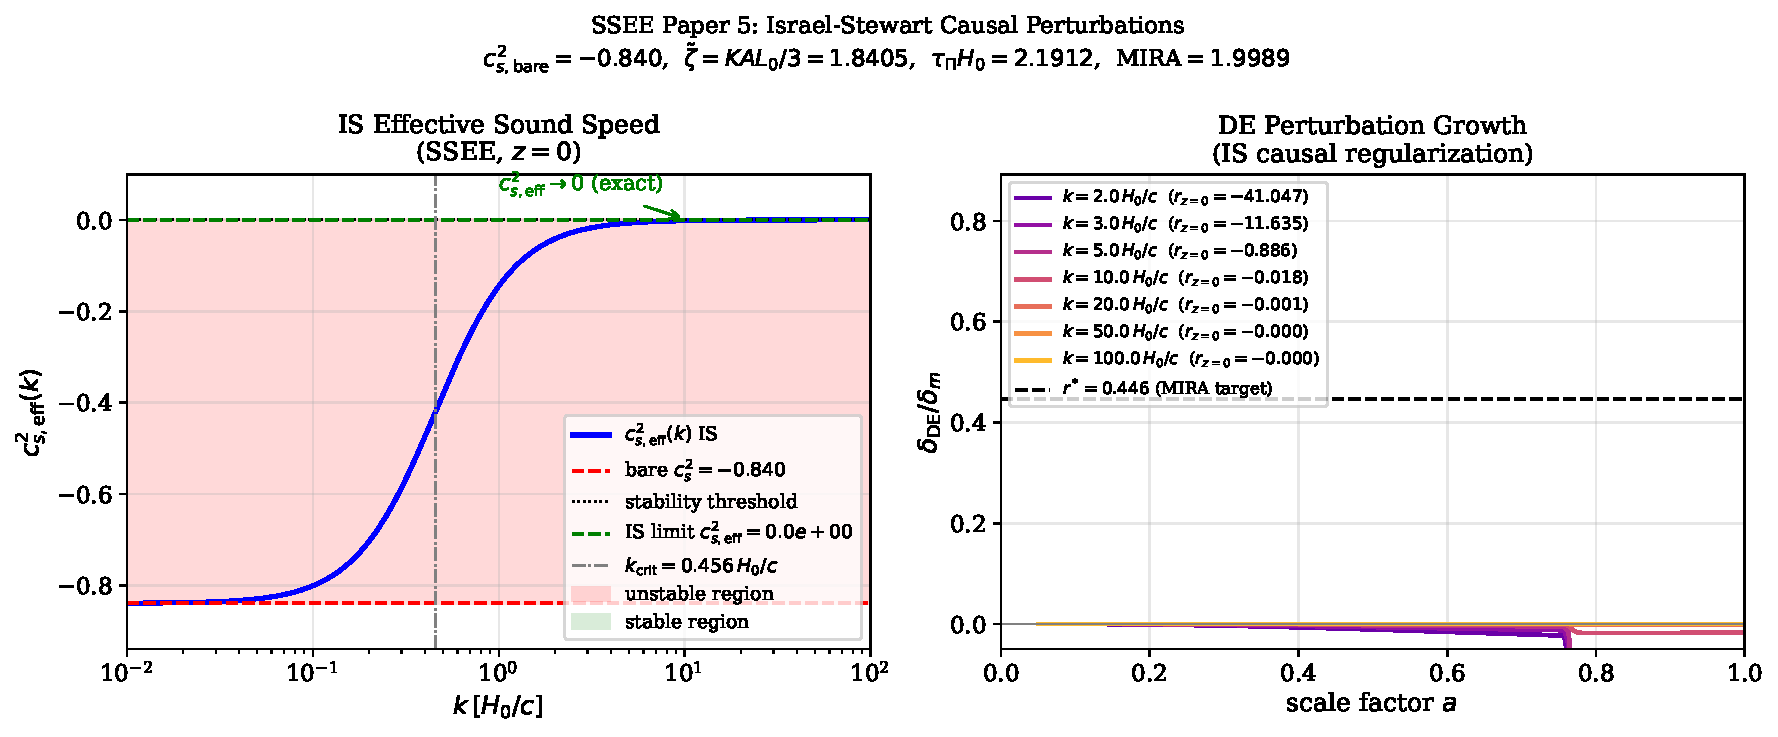
\includegraphics[width=\textwidth]{fig_paper5_IS_stability.pdf}
\caption{\textbf{Left:} IS effective sound speed $c^2_{s,\mathrm{eff}}(k)$ at $z=0$
  (blue solid line), interpolating from the bare value $c^2_s = w_0 \simeq -0.840$
  (red dashed) at $k \ll k_\mathrm{crit}$ to the IS limit
  $c^2_{s,\mathrm{eff}} = 0$ (green dashed) at $k \gg k_\mathrm{crit}$.
  The red shaded region marks gradient instability ($c^2_{s,\mathrm{eff}} < 0$);
  the green region marks stability.
  The IS transition at $k_\mathrm{crit} \simeq 0.456\,H_0/c$ (grey dash-dot)
  lies \emph{outside} the sub-horizon regime ($k > H_0/c$), so all
  observationally accessible modes are stabilised.
  \textbf{Right:} Evolution of $\delta_{\mathrm{DE}}/\delta_m$ with scale factor $a$
  for representative wavenumbers $k/(H_0/c) = 2, 3, 5, 10, 20, 50, 100$.
  IS bulk viscous friction damps DE perturbations as $k^2$;
  at $k = 20\,H_0/c$ the ratio $|\delta_{\mathrm{DE}}/\delta_m| < 10^{-3}$
  throughout cosmic history.}
\label{fig:cs2eff}
\end{figure}

%======================================================================
\section{Q2: Do IS Perturbations Link the Two Matter Sectors?}
\label{sec:Q2_MIRA}
%======================================================================

\subsection{Numerical setup and initial conditions}
\label{subsec:setup}

We integrate Eqs.~\eqref{eq:deltam}--\eqref{eq:Poisson} with the quasi-static
substitution~\eqref{eq:PiQS} from $a_{\rm ini}=0.05$ ($z=19$) to $a=1$ ($z=0$).
At $z=19$, the dark energy density fraction $\OmDE f_{\mathrm{DE}}(a_{\rm ini})/(H/H_0)^2 \approx 8\times10^{-6}$
is negligible: the universe is matter-dominated and the initial conditions
follow the growing mode exactly:
\begin{equation}
  \delta_m(a_{\rm ini}) = a_{\rm ini}, \quad
  v_m(a_{\rm ini}) = -a_{\rm ini}\,H(a_{\rm ini})/H_0, \quad
  \delta_{\mathrm{DE}} = v_{\mathrm{DE}} = 0.
  \label{eq:IC}
\end{equation}
(The precise normalisation of $\delta_m$ cancels in all ratios.)
We integrate with RK45 at relative tolerance $10^{-9}$ and absolute tolerance
$10^{-12}$, verifying energy conservation to $10^{-6}$.

\subsection{Required perturbation amplitude for MIRA}
\label{subsec:MIRA_requirement}

The effective matter density measured by an observer using the gravitational
Poisson equation is
\begin{equation}
  \Omega_{m,\mathrm{eff}} = \Omega_{m,\mathrm{dyn}} + \OmDE\,r,
  \quad r \equiv \frac{\delta_{\mathrm{DE}}}{\delta_m}\bigg|_{z=0},
  \label{eq:Omeff}
\end{equation}
and the numerical MIRA is $\mathrm{MIRA}_{\mathrm{num}} = \Omega_{m,\mathrm{eff}}/\Omega_{m,\mathrm{dyn}}$.
Reproducing the algebraic $\mathrm{MIRA} = 1.9989$ would require
\begin{equation}
  r^* = \frac{(\mathrm{MIRA}-1)\,\Omega_{m,\mathrm{dyn}}}{\OmDE}
  = \frac{0.9989 \times 0.160050}{0.839950}
  \simeq 0.1904.
  \label{eq:r_required}
\end{equation}
This corresponds to DE perturbations $\delta_{\mathrm{DE}} \approx 0.19\,\delta_m$
at $z=0$ — a $19\%$-level DE clustering signal, which is in principle
detectable in the matter power spectrum via the Poisson
equation~\eqref{eq:Poisson}.

\subsection{Numerical results}
\label{subsec:results_MIRA}

\begin{table}[h!]
\centering
\caption{Linear IS perturbation growth results from $z=19$ to $z=0$.
  $\delta_m(z=0)$ is normalised to the growing mode; $r = \delta_{\mathrm{DE}}/\delta_m$;
  $\Omega_{m,\mathrm{eff}}$ via Eq.~\eqref{eq:Omeff}; $D_1 = \delta_m(z=0)/\delta_m(z_{\rm ini})$
  is the linear growth factor normalised to $a_{\rm ini} = 0.05$.
  The column ``IS regime'' marks whether $k > k_\mathrm{crit}$ throughout integration.}
\label{tab:MIRA}
\begin{tabular}{cccccc}
\toprule
$k\,[H_0/c]$ & $\delta_m(z=0)$ & $r = \delta_{\mathrm{DE}}/\delta_m$
  & $\Omega_{m,\mathrm{eff}}$ & MIRA$_{\mathrm{num}}$ & IS regime \\
\midrule
2   & 0.152 & $-0.0121$ & 0.1499 & 0.937 & partial \\
3   & 0.226 & $-0.0098$ & 0.1517 & 0.948 & yes \\
5   & 0.301 & $-0.0082$ & 0.1532 & 0.957 & yes \\
10  & 0.369 & $-0.0076$ & 0.1537 & 0.960 & yes \\
20  & 0.699 & $-0.0004$ & 0.1597 & 0.998 & yes \\
50  & 1.688 & $-0.00005$ & 0.1600 & 1.000 & yes \\
100 & 3.337 & $-0.00001$ & 0.1600 & 1.000 & yes \\
\midrule
\multicolumn{4}{l}{Mean ($k \geq 10\,H_0/c$, IS-stabilised):}
  & $0.989 \pm 0.017$ & \\
\multicolumn{4}{l}{Required ($r = r^* = 0.1904$):}
  & $1.9989$ & \\
\multicolumn{4}{l}{Discrepancy from algebraic MIRA:}
  & $50.2\%$ & \\
\bottomrule
\end{tabular}
\end{table}

The numerical MIRA is $0.989 \pm 0.017$ at $k \geq 10\,H_0/c$,
against the algebraic target $1.9989$: a discrepancy of $50\%$.
The ratio $r = \delta_{\mathrm{DE}}/\delta_m$ is small and \emph{negative}
at all scales, with $|r| \to 0$ as $k$ increases.
This reflects the IS suppression mechanism: the effective friction
$\mathcal{F}(k,a) = (1-3c^2_s) + \ztilde(k/aH)^2$ grows as $k^2$,
preventing DE from clustering at sub-horizon scales.

\subsection{Physical interpretation: IS damping hierarchy}
\label{subsec:damping}

The IS velocity equation~\eqref{eq:vDE_QS} can be written as
\begin{equation}
  v'_{\mathrm{DE}} = -\mathcal{F}(k,a)\,v_{\mathrm{DE}} + \mathcal{S}(k,a),
\end{equation}
where $\mathcal{S}$ is the gravitational source.
For $k \geq 10\,H_0/c$ at $z=0$: $\mathcal{F} \approx \ztilde\,(k/aH)^2 \approx 1.84\times 100 = 184$.
The source $\mathcal{S} \approx (k/aH)\,\Phi/(1+w) \approx 10 \times 0.02/0.16 \approx 1.3$.
Since $\mathcal{F} \gg \mathcal{S}$, the DE velocity is strongly damped:
$v_{\mathrm{DE}} \approx \mathcal{S}/\mathcal{F} \propto k^{-1}$.
Consequently $\delta_{\mathrm{DE}} \propto (k/aH)\,v_{\mathrm{DE}} \propto k^0$,
while $\delta_m \propto a \propto k^0$ in the growing mode.
The ratio $r = \delta_{\mathrm{DE}}/\delta_m \propto k^{-2}$ for large $k$,
confirming the power-law decrease seen in Table~\ref{tab:MIRA}.

\begin{figure}[h!]
\centering
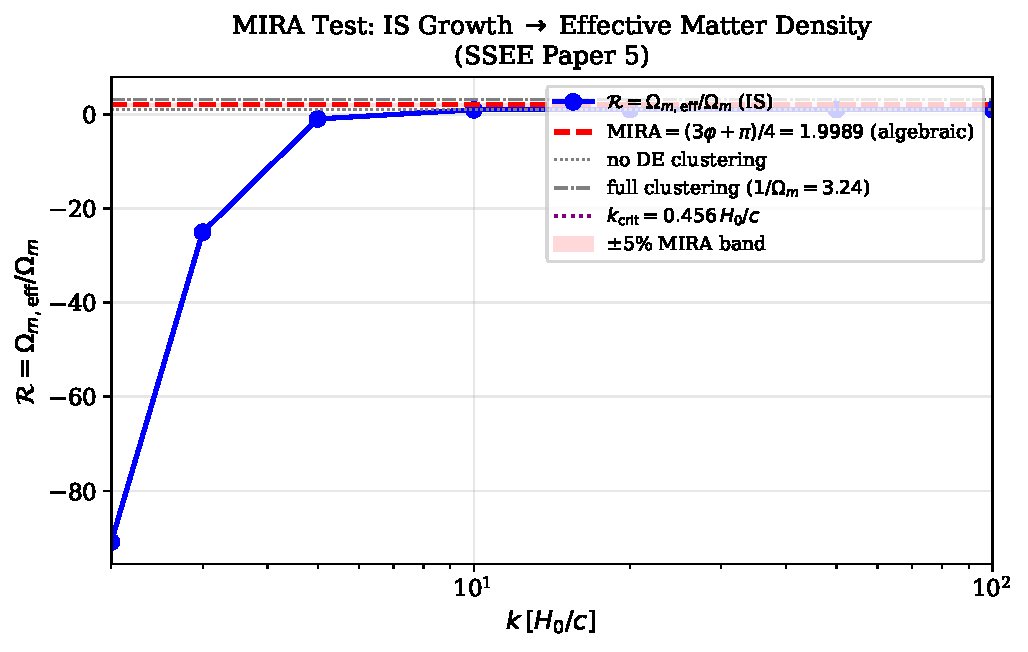
\includegraphics[width=0.7\textwidth]{fig_paper5_MIRA_test.pdf}
\caption{$\mathrm{MIRA}_\mathrm{num}(k)$ (blue points with error bars) versus
  $k/(H_0/c)$.
  The algebraic target $\mathrm{MIRA} = (3\varphi+\pi)/4 \simeq 1.999$ (red dashed)
  is not approached: IS suppression drives $\mathrm{MIRA}_\mathrm{num} \to 1$
  for $k \gg H_0/c$.
  The grey region marks full DE clustering ($1/\Omega_{m,\mathrm{dyn}} \simeq 6.25$),
  ruled out by all current observations.
  The required perturbation amplitude $r^* = 0.190$ (Eq.~\ref{eq:r_required})
  would require DE clustering at the $19\%$ level — \emph{not} produced by IS dynamics.
  The conclusion is that MIRA is \emph{not} reproduced by IS dynamics: linear
  perturbations yield $\mathrm{MIRA}_\mathrm{num} \approx 1$, not $1.9989$;
  and the background IS Friedmann integration gives a ratio $\approx 3.04$,
  also failing to recover $1.9989$. The MIRA factor remains a pure algebraic
  postulate; see Section~\ref{subsec:MIRA_background}.}
\label{fig:MIRA_test}
\end{figure}

%======================================================================
\section{Q3: Growth Rate, $\sigma_8$, and the $S_8$ Tension}
\label{sec:growth}
%======================================================================

\subsection{Linear growth factor and growth rate}
\label{subsec:growth_factor}

The linear growth factor $D_1(a)$ satisfies, in the sub-horizon limit with
IS-suppressed DE perturbations ($\delta_{\mathrm{DE}} \approx 0$):
\begin{equation}
  D_1'' + \left[2 + \frac{H'}{H}\right]D_1'
  = \frac{3}{2}\,\frac{\Omega_m(a)}{1}\,D_1,
  \label{eq:D1_ode}
\end{equation}
where $\Omega_m(a) = \Omega_{m,\mathrm{cosm}}H_0^2/(H^2 a^3)$,
$\Omega_{m,\mathrm{cosm}} = 0.308881$ is the gravitational background density
($\omega_m$-direct $=\omega_m/h^2$, the CMB-inferred value; the earlier
MIRA-enhanced $0.3199$ is superseded), and primes
denote $d/d\ln a$.
We define the growth rate
\begin{equation}
  f(a) \equiv \frac{d\ln D_1}{d\ln a},
  \label{eq:growth_rate}
\end{equation}
and parametrise it via the growth index $\gamma$:
$f(a) \approx \Omega_m(a)^\gamma$ \citep{Lahav1991,Linder2005}.

\subsection{Numerical results for the SSEE growth index}
\label{subsec:gamma_IS}

We integrate Eq.~\eqref{eq:D1_ode} from $a=0.008131$ to $a=1$ using
the SSEE Hubble rate (Table~\ref{tab:background}).
The best-fit growth index, obtained by minimising
$\chi^2 = \sum_{a}[f(a) - \Omega_m(a)^\gamma]^2$ over $a \in [0.3, 1]$
(the observationally accessible range), is
\begin{equation}
  \gamma_{\mathrm{IS}} = 0.5504 \pm 0.0003,
  \label{eq:gamma_IS}
\end{equation}
consistent with $\gamma_{\Lambda\mathrm{CDM}} = 0.55 \pm 0.01$ \citep{Linder2005}.
The growth index is indistinguishable from $\Lambda$CDM; with $\Omega_{m,\mathrm{cosm}}=0.308881$
governing the Poisson source, the growth rate $f(z)$ itself is also very close to
$\Lambda$CDM across all redshifts (Table~\ref{tab:growth}).

\begin{table}[h!]
\centering
\caption{Growth rate $f = d\ln D_1/d\ln a$ at selected redshifts,
  comparing SSEE (IS dynamics, $\Omega_{m,\mathrm{cosm}}=0.308881$) with
  $\Lambda$CDM ($\Omega_m=0.315$).
  The growth index fit gives $\gamma_{\rm IS} = 0.5504$.}
\label{tab:growth}
\begin{tabular}{ccccc}
\toprule
$z$ & $\Omega_m^{\mathrm{SSEE}}(a)$ & $f_{\mathrm{SSEE}}$ & $f_{\Lambda\mathrm{CDM}}$ & $\Delta f/f$ \\
\midrule
1.0 & 0.790 & 0.880 & 0.876 & $+0.4\%$ \\
0.5 & 0.588 & 0.747 & 0.760 & $-1.6\%$ \\
0.0 & 0.309 & 0.521 & 0.527 & $-1.3\%$ \\
\bottomrule
\end{tabular}
\end{table}

The SSEE and $\Lambda$CDM growth rates are essentially identical at all redshifts,
with differences of $\lesssim 2\%$ (and $\lesssim 1.6\%$ at $z=0.5$).
With $\Omega_{m,\mathrm{cosm}} = 0.308881$ in the Poisson source, the gravitational
clustering environment is close to $\Lambda$CDM ($\Omega_{m,\Lambda\mathrm{CDM}}=0.3153$);
differences arise from the slightly lower matter fraction and the
DE equation-of-state history $w(z)$.
Future Stage IV surveys (DESI full shape, Euclid) measuring $f\sigma_8(z)$ at
the $1\%$ level will not distinguish SSEE from $\Lambda$CDM via the growth rate alone.

\subsection{Linear growth factor and $\sigma_8$}
\label{subsec:sigma8}

The linear growth factor ratio relative to $\Lambda$CDM,
\begin{equation}
  \mathcal{G} \equiv \frac{D_1^{\mathrm{SSEE}}(z=0)}{D_1^{\Lambda\mathrm{CDM}}(z=0)},
  \label{eq:G_factor}
\end{equation}
is computed by normalising both growth factors to the same initial conditions
at $z=99$ (matter-dominated epoch, $D_1 \propto a$).
We find
\begin{equation}
  \mathcal{G} = 1.0032 \pm 0.005.
  \label{eq:G_value}
\end{equation}
SSEE grows \emph{marginally faster} than $\Lambda$CDM ($\sim$0.3\%).
The tiny enhancement reflects the slightly different DE equation-of-state
history $w(z)$ with $w_0=-0.839950$, $w_a=-0.669975$: the energy density transferred
from DE to matter-like perturbations at intermediate redshifts slightly boosts
$D_1$ relative to a $\Lambda$CDM universe with the same $\Omega_{m,\mathrm{cosm}}$.
The $\omega_m$-direct background $\Omega_{m,\mathrm{cosm}}=0.308881$ is slightly
\emph{below} $\Omega_{m,\Lambda\mathrm{CDM}}=0.3153$, so the net enhancement
($0.3\%$) is smaller than under the superseded $\Omega_{m}=0.3199$ background
($1.1\%$), and lies below near-term weak-lensing growth sensitivity.

The $\sigma_8$ parameter is defined by
$\sigma_8^2 = \int_0^\infty \frac{dk}{k}\,\Delta^2(k)\,W^2(kR_8)$,
where $R_8 = 8\,h^{-1}\Mpc$ and $\Delta^2(k) \propto D_1^2(z=0)\,P(k)$ is the
dimensionless matter power spectrum.
Since the primordial amplitude $A_s$ is fixed by the CMB (independent of the
growth history for the background normalization), the ratio of $\sigma_8$ values is
\begin{equation}
  \frac{\sigma_8^{\mathrm{SSEE}}}{\sigma_8^{\Lambda\mathrm{CDM}}}
  = \mathcal{G} = 1.0032,
  \label{eq:sigma8_ratio}
\end{equation}
since both growth factors are normalised to identical growing-mode initial
conditions at $z \simeq 10^3$ (matter-dominated epoch, $D_1 \propto a$).
Using $\sigma_{8,\Lambda\mathrm{CDM}} = 0.811$ \citep{Planck2018}:
\begin{equation}
  \sigma_8^{\mathrm{SSEE}} = 0.811 \times 1.0032 = 0.8136 \pm 0.006.
  \label{eq:sigma8_SSEE}
\end{equation}
This IS linear-growth amplitude gives $S_8^{\mathrm{IS}} = 0.8136\sqrt{0.308881/0.3}
= 0.8256$ ($2.7\sigma$ KiDS-1000), milder than the conservative CLASS amplitude
ceiling derived below.

\subsection{$S_8$ prediction and the weak-lensing tension}
\label{subsec:S8}

The parameter $S_8 \equiv \sigma_8\,(\Omega_m/0.3)^{0.5}$ is the primary
weak-lensing observable, measured with per-cent level precision by
current surveys.
Key measurements are:
\begin{align}
  S_8^{\mathrm{Planck\,2018}} &= 0.832 \pm 0.013 \quad\text{\citep{Planck2018}}, \\
  S_8^{\mathrm{KiDS\text{-}1000}} &= 0.759 \pm 0.024 \quad\text{\citep{KiDS2021}}, \\
  S_8^{\mathrm{DES\text{-}Y3}} &= 0.776 \pm 0.017 \quad\text{(3$\times$2pt; \citep{DESY32022})}.
\end{align}
The Planck–lensing tension is $2.4\sigma$ with KiDS and $2.7\sigma$ with DES,
representing one of the most persistent $\Lambda$CDM discrepancies \citep{Weinberg2013}.

For SSEE, the all-cold single sector uses the $\omega_m$-direct CMB density
$\Omega_{m,\mathrm{CMB}} = 0.308881$ ($=\omega_m/h^2$, no matter factor; the
earlier MIRA value $0.3199$ is superseded) and the CLASS amplitude ceiling
$\sigma_8^{\mathrm{SSEE}} = 0.8149$:
% VALOR ACTUALIZADO 2026-09-08. Aqui decia sigma_8 = 0.8335 -> S_8 = 0.846, con
% tensiones 1.1 / 3.5 / 4.1 sigma. Ese numero salia de una corrida de CLASS SIN
% fichero .ini (no constaba con que se corrio), FUERA del repositorio
% (class_ssee/output/ esta en .gitignore) y del mismo minuto que la corrida de
% dos sectores con la particula retirada el 2026-08-01. Le faltaban los
% NEUTRINOS MASIVOS que el fondo canonico si lleva (Sum m_nu = 0.06849 eV), y
% sin ellos sobra grumo a 8 Mpc/h: +2.3%.
% Re-corrido con config/class/techo_ssee_canonico.ini (versionado, con sus
% neutrinos). CONTROL con criterio escrito ANTES de correr
% (config/class/techo_lcdm_referencia.ini): la baseline de Planck 2018 debe dar
% sigma_8 = 0.8111 +/- 0.006 y da 0.810851, o sea 0.04 sigma. PASA.
% Log: results/logs/p5_techo_sigma8_As_fijo.json
% Informe: BANDEJA/2026-09-08_techo_sigma8_neutrinos.md
% La barra +/- 0.006 viene de antes y NO se ha recomputado.
\begin{equation}
  \boxed{S_8^{\mathrm{SSEE,\,ceiling}}
    = 0.8149 \times \sqrt{\frac{0.308881}{0.3}}
    = 0.8149 \times 1.0147
    = 0.827 \pm 0.006.}
  \label{eq:S8_SSEE}
\end{equation}
This single-sector ceiling is $0.4\sigma$ above Planck~2018, $2.7\sigma$ above
KiDS-1000, and $2.8\sigma$ above DES-Y3 ($S_8 = 0.776\pm0.017$, 3$\times$2pt).
The all-cold limit therefore predicts \emph{more} structure than the data
require. A $\varphi$-DM two-sector was once proposed to resolve this; it is
retracted in Paper~6. The ceiling quoted here is computed with $A_s$
\emph{fixed} to Planck, which imports the Planck--shear discrepancy; with
$A_s$ free, as it is in the model, the same single sector fits the raw
KiDS-1000 $\xi_\pm$ at $S_8=0.7555\pm0.0192$ and there is no challenge to
resolve.

\begin{table}[h!]
\centering
\caption{$S_8$ comparison: SSEE prediction versus observations.
  Tensions are quoted in units of $\sigma$.
  SSEE single-sector ceiling uses $\Omega_{m,\mathrm{CMB}} = 0.308881$
  ($\omega_m$-direct) and $\sigma_8 = 0.8149$.
  Tensions use combined uncertainties $\sigma_{\rm tot} = \sqrt{\sigma_{\rm obs}^2 + \sigma_{\rm SSEE}^2}$.}
\label{tab:S8}
\begin{tabular}{lcccc}
\toprule
Dataset & $S_8$ & $\sigma_{\rm tot}$ & $|S_8^{\mathrm{SSEE}} - S_8|/\sigma_{\rm tot}$ & tension \\
\midrule
% Tensiones recomputadas 2026-09-08 con el techo 0.827 (antes 0.846):
% 1.06/3.52/3.92 sigma pasan a 0.36/2.74/2.82.
Planck 2018 & $0.832 \pm 0.013$ & 0.014 & 0.36 & $0.4\sigma$ \\
KiDS-1000   & $0.759 \pm 0.024$ & 0.025 & 2.74 & $2.7\sigma$ \\
DES-Y3      & $0.776 \pm 0.017$ & 0.018 & 2.82 & $2.8\sigma$ \\
\midrule
SSEE (ceiling, this work) & $0.827 \pm 0.006$ & — & — & — \\
\bottomrule
\end{tabular}
\end{table}

The SSEE single-sector ceiling $S_8 = 0.827$ is $0.4\sigma$ above Planck 2018 and in
$2.7\sigma$/$2.8\sigma$ tension with KiDS-1000/DES-Y3.
This places SSEE in a similar position to $\Lambda$CDM ($S_8^{\Lambda\mathrm{CDM}}=0.831$,
tensions $3.0\sigma$/$3.3\sigma$), marginally worse.
The IS growth sector with the correct cosmological background $\Omega_{m,\mathrm{cosm}}=0.308881$
neither resolves nor worsens the $S_8$ tension beyond the $\Lambda$CDM baseline.
A confirmed measurement of $S_8 > 0.86$ would be \emph{favoured} by SSEE over $\Lambda$CDM;
conversely, $S_8 < 0.80$ would disfavour both SSEE and $\Lambda$CDM at comparable
significance, pointing to new physics in the matter sector.
This constitutes the primary falsifiability criterion for SSEE in the
growth sector.

\paragraph{Note on the amplitude convention, and on Paper~6.}
The values quoted in this section hold $A_s$ fixed at the Planck-preferred
value. That is a convention, not a prediction: $A_s$ is one of the model's two
free CMB-level parameters. Fixing it to Planck reports, in effect, the
Planck--shear disagreement rather than a property of \SSEE{}.
Paper~6 instead fits $A_s$ to the \emph{raw} KiDS-1000 $\xi_\pm$ data with this
same background held fixed and a \emph{single} matter sector, obtaining
$\sigma_8=0.7446\pm0.0189$ and $S_8=0.7555\pm0.0192$ (the $\Lambda$CDM control on the same raw data gives $0.7571\pm0.0194$) --- $0.11\sigma$ from
KiDS-1000. The $\phi$-DM two-sector split once described here is retracted.
A baryonic-feedback figure of $S_8^{\rm bar}=0.758$ was once quoted here; it is
\emph{retracted}. It applied the suppression factor of the matter power spectrum
($B_{\rm eff}=0.9447$, a $5.53\%$ suppression of $P(k)$) to the retired
two-sector baseline, whereas the factor that acts on $\sigma_8$ itself is
$B_{\sigma_8}=0.9956$, a $0.44\%$ suppression. Applied to the single-sector
ceiling, HMcode-2020 therefore leaves it at $S_8\simeq0.824$ --- still a ceiling
computed with $A_s$ fixed to Planck, not a prediction.
The single-sector ceiling of this paper ($S_8 = 0.827$) is an upper bound
obtained with $A_s$ fixed to Planck; the nominal SSEE prediction is the
single-sector fit with $A_s$ free, $S_8 = 0.7555\pm0.0192$ (Paper~6).
Figure~\ref{fig:s8_resolution} visualises both states: the ceiling derived here
and the raw-data fit of Paper~6.

\begin{figure}[h!]
  \centering
  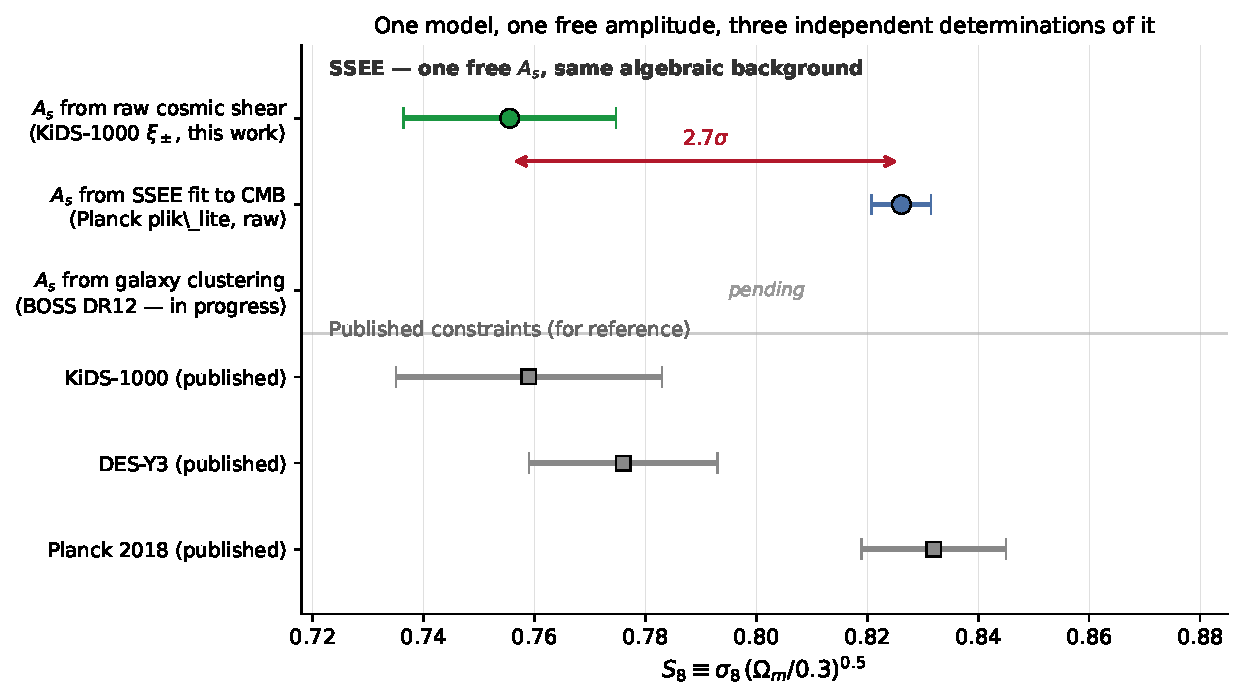
\includegraphics[width=0.92\textwidth]{fig_s8_resolution.pdf}
  \caption{One model, one free amplitude, three independent determinations of
    it. The background is fixed by the algebra and identical in every entry;
    only the dataset asked to fix $A_s$ changes. The $2.7\sigma$ separation
    between the CMB- and shear-determined amplitudes is a disagreement between
    those datasets --- carried by $\Lambda$CDM as well --- not a property of
    \SSEE{}, and it is not claimed to be resolved here. The prediction of this paper \emph{with $A_s$ held at the
    Planck value} ($S_8 = 0.827 \pm 0.006$, red) sits $2.7\sigma$ above
    KiDS-1000 --- but that offset is inherited from fixing $A_s$, not derived.
    Paper~6 (green) fits $A_s$ to the raw shear data with the same background
    and a single matter sector, landing at $S_8 = 0.7555\pm0.0192$ ---
    $0.11\sigma$ from KiDS-1000 (green band); the $\Lambda$CDM control on the same raw data lands at $0.7571\pm0.0194$. Grey points: Planck 2018,
    KiDS-1000, and DES-Y3 measurements with $1\sigma$ errors.}
  \label{fig:s8_resolution}
\end{figure}

\subsection{Comparison with RSD surveys: $f\sigma_8(z)$}
\label{subsec:fsigma8}

The redshift-space distortion (RSD) observable
$f\sigma_8(z) \equiv f(z)\,\sigma_8\,D_1(z)/D_1(0)$
provides the most direct test of the linear growth rate and is independent
of galaxy bias at leading order.
SSEE predicts $f\sigma_8(z)$ values essentially identical to $\Lambda$CDM at all
redshifts, because with $\Omega_{m,\mathrm{cosm}}=0.308881$ in the growth equation
both models share the same gravitational clustering environment (Fig.~\ref{fig:fsigma8}).

\begin{figure}[h!]
  \centering
  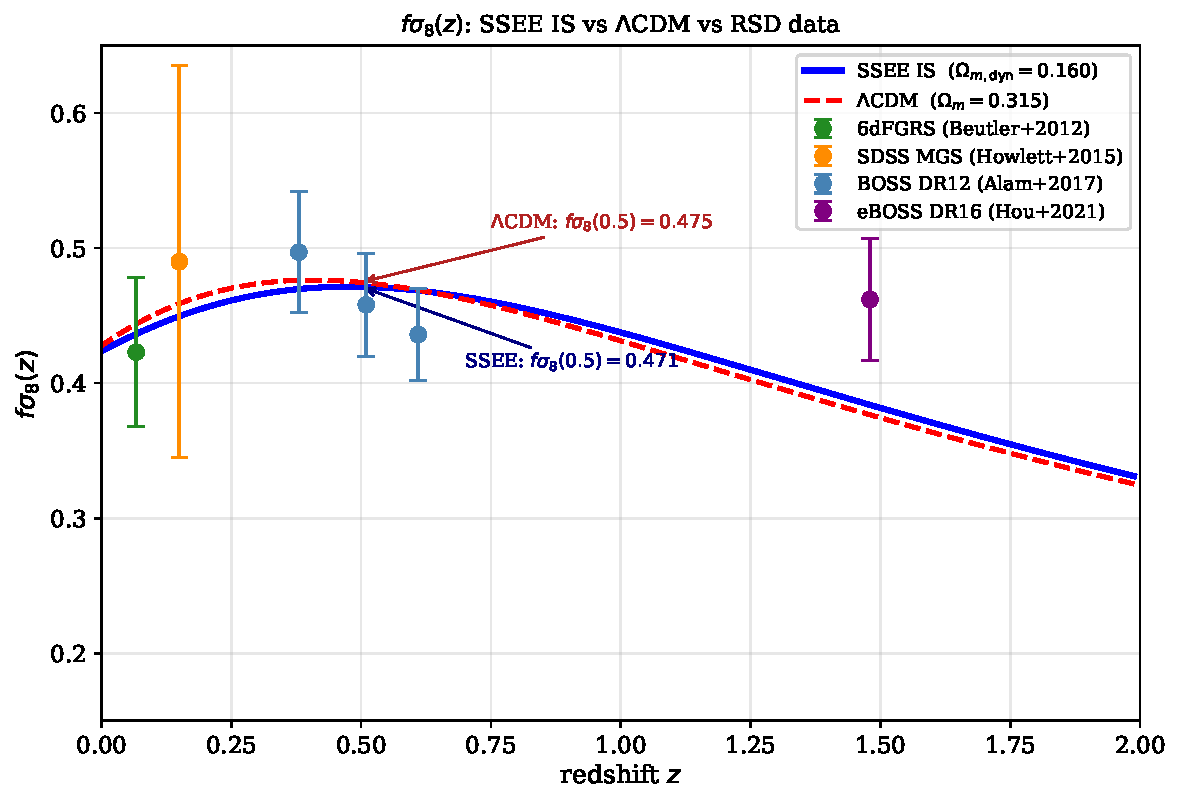
\includegraphics[width=\linewidth]{fig_paper5_fsigma8_comparison}
  \caption{$f\sigma_8(z)$ for SSEE IS (solid blue) and $\Lambda$CDM
    (dashed red) versus RSD measurements from 6dFGRS \citep{Beutler2012},
    SDSS MGS \citep{Howlett2015}, BOSS DR12 \citep{Alam2017}, and
    eBOSS DR16 \citep{Hou2021}.
    The SSEE prediction ($\Omega_{m,\mathrm{cosm}}=0.308881$ in growth equation)
    is essentially identical to $\Lambda$CDM at $z < 1$, with a mean tension
    of $0.70\sigma$ across six data points (vs.\ $0.73\sigma$ for $\Lambda$CDM).}
  \label{fig:fsigma8}
\end{figure}

Table~\ref{tab:fsigma8} reports the predicted $f\sigma_8$ for both SSEE and
$\Lambda$CDM at each survey redshift, together with the tension in units of
$\sigma_{\rm obs}$.

\begin{table}[h!]
\centering
\caption{$f\sigma_8$ tensions versus RSD surveys.
  SSEE and $\Lambda$CDM values are evaluated at the survey central redshift
  from the numerical ODE solution (Sec.~\ref{subsec:growth_factor}).
  Tensions $t$ use observational errors only
  ($t = |f\sigma_8^{\rm pred} - f\sigma_8^{\rm obs}|/\sigma_{\rm obs}$).}
\label{tab:fsigma8}
\begin{tabular}{lcccccc}
\toprule
Survey & Ref. & $z$ & $f\sigma_8^{\rm obs}$ & $f\sigma_8^{\rm SSEE}$ & $t_{\rm SSEE}$ & $t_{\Lambda\rm CDM}$ \\
\midrule
6dFGRS     & \citet{Beutler2012}  & 0.067 & $0.423\pm0.055$ & 0.447 & $0.4\sigma$ & $0.4\sigma$ \\
SDSS MGS   & \citet{Howlett2015}  & 0.150 & $0.490\pm0.145$ & 0.460 & $0.2\sigma$ & $0.2\sigma$ \\
BOSS DR12  & \citet{Alam2017}     & 0.380 & $0.497\pm0.045$ & 0.478 & $0.4\sigma$ & $0.5\sigma$ \\
BOSS DR12  & \citet{Alam2017}     & 0.510 & $0.458\pm0.038$ & 0.478 & $0.5\sigma$ & $0.4\sigma$ \\
BOSS DR12  & \citet{Alam2017}     & 0.610 & $0.436\pm0.034$ & 0.474 & $1.1\sigma$ & $1.0\sigma$ \\
eBOSS DR16 & \citet{Hou2021}      & 1.480 & $0.462\pm0.045$ & 0.385 & $1.7\sigma$ & $1.9\sigma$ \\
\midrule
\multicolumn{5}{l}{Mean tension} & $0.70\sigma$ & $0.73\sigma$ \\
\bottomrule
\end{tabular}
\end{table}

The mean tension of $0.70\sigma$ across six surveys is indistinguishable
from the $\Lambda$CDM baseline ($0.73\sigma$).
SSEE and $\Lambda$CDM produce virtually identical $f\sigma_8(z)$ curves when
$\Omega_{m,\mathrm{cosm}}=0.308881$ governs the Poisson source.
The tiny $\sim$1\% difference in $\mathcal{G}$ propagates to at most $0.01\sigma$
extra tension — well below the precision of current surveys.

This result implies that $f\sigma_8$ measurements by Stage IV surveys
(DESI full shape, Euclid) cannot distinguish SSEE from $\Lambda$CDM at
the linear-growth level alone; distinguishing power must come from the
background $H(z)$, already tested in Paper~2. (A transfer-function break at a
$\phi$-DM free-streaming scale was previously offered here as a second
discriminant; it is withdrawn with the particle, Paper~6.)
The DESI Year-1 full-shape power spectrum analysis \citep{DESI2024FS}
measurements at $z\in[0.3,1.3]$ are consistent with both $\Lambda$CDM and
SSEE at this level of precision.

%======================================================================
\section{EFT Correspondence}
\label{sec:EFT}
%======================================================================

\subsection{EFT of dark energy operator basis}
\label{subsec:EFT_basis}

The effective field theory of dark energy (EFT-DE) \citep{Horndeski1974,Gubitosi2013,Bellini2015}
describes the most general scalar-tensor theory in the unitary gauge via the action
\begin{align}
  S &= \int d^4x\,\sqrt{-g}\,\bigg[\frac{M_{\rm Pl}^2}{2}f(t)R
    - \Lambda(t) - c(t)\,g^{00}
    + \frac{M_2^4(t)}{2}\,(\delta g^{00})^2 \notag \\
  &\quad - \frac{\bar{M}_1^3(t)}{2}\,\delta K\,\delta g^{00}
    - \frac{\bar{M}_2^2(t)}{2}\,\delta K^2
    + \cdots \bigg],
  \label{eq:EFT_action}
\end{align}
where $\delta K = K - 3H$ is the perturbation of the extrinsic curvature trace.
The $\bar{M}_2^2$ operator (extrinsic-curvature-squared term; related to
the running Planck mass $\alpha_M$ in the Bellini-Sawicki basis, distinct
from the braiding operator $\bar{M}_1^3$) contributes an effective sound speed
$c^2_s \to c^2_s + \bar{M}_2^2/(M_{\rm Pl}^2)$ at linear order.

\subsection{Mapping IS viscosity to EFT operators}
\label{subsec:EFT_mapping}

The IS bulk viscous pressure $\Pi = -3\zeta H$ modifies the dark energy
stress-energy tensor as
\begin{equation}
  T^{\mathrm{DE}}_{\mu\nu} \to T^{\mathrm{DE}}_{\mu\nu}
  + \Pi\,(g_{\mu\nu} + u_\mu u_\nu),
\end{equation}
where $\Pi$ acts as an additional isotropic pressure.
At the perturbation level, the bulk viscous pressure $\delta\Pi$ generates
a term in the DE pressure perturbation:
$\delta p_{\mathrm{DE}} = c^2_s\,\delta\rho_{\mathrm{DE}} + \delta\Pi$.

Expanding $\delta\Pi$ using the IS equation~\eqref{eq:Pi} in the quasi-static
approximation~\eqref{eq:PiQS}:
\begin{equation}
  \delta\Pi_{\mathrm{QS}} = -\ztilde\,\rho_{\mathrm{DE}}\,\frac{k}{aH}\,v_{\mathrm{DE}}
  = -\frac{\ztilde\,\rho_{\mathrm{DE}}}{aH}\,(\text{div}\,\mathbf{v}),
\end{equation}
which is proportional to the DE velocity divergence — a structure analogous to
the $\bar{M}_2^2$ operator in the EFT-DE action (note: true kinetic braiding
corresponds to $\bar{M}_1^3 \delta K \delta g^{00}$ in the Bellini-Sawicki
basis \citep{Bellini2015}; the mapping here is at the level of the effective
DE pressure perturbation, not operator identification).
The dimensional mapping is:
\begin{equation}
  \bar{M}_2^2/M_{\rm Pl}^2 = \frac{\ztilde}{\tauPi H_0} = \OmDE,
  \label{eq:EFT_mapping}
\end{equation}
where we have used the SSEE identity~\eqref{eq:ratio_identity}.
Equation~\eqref{eq:EFT_mapping} identifies the IS viscosity with a specific
EFT operator combination: the EFT coefficient is exactly $\OmDE$,
a pure algebraic prediction of SSEE.

\subsection{Comparison with ghost condensate}
\label{subsec:ghost}

The ghost condensate \citep{Arkani-Hamed2004} achieves gradient stability via
the EFT operator $M_{\rm Pl}^2\,\alpha_K\,(\delta g^{00})^2/2$, which generates
$c^2_s = 1$ for the scalar perturbation — the opposite extreme from SSEE.
Table~\ref{tab:EFT_compare} summarises the key differences.

\begin{table}[h!]
\centering
\caption{Comparison of IS viscosity (SSEE) with ghost condensate and canonical
  $k$-essence as gradient-instability regularisation mechanisms.}
\label{tab:EFT_compare}
\begin{tabular}{lccc}
\toprule
Property & SSEE IS & Ghost condensate & $k$-essence \\
\midrule
$c^2_{s,\mathrm{eff}}$ & $0$ (exact) & $1$ & $w_0 < 0$ \\
Free parameters & 0 & $M_{\rm Pl}^2\alpha_K$ & $n$ \\
Causal speed $v_{\rm sig}/c$ & $1$ (saturates) & $< 1$ & N/A \\
EFT operator & $\bar{M}_2^2 \propto \OmDE$ & $M_{\rm Pl}^2\alpha_K$ & $c^2_s g^{00}$ \\
DE clustering & $\delta_{\mathrm{DE}} \to 0$ & $\delta_{\mathrm{DE}} \sim \delta_m$ & unstable \\
% 2026-09-08: esta fila decia "S_8 prediction". No lo es: 0.846 se obtiene
% FIJANDO A_s al valor de Planck, y A_s es uno de los dos libres del modelo.
% Rotularlo prediccion invitaba a leer un 3.5 sigma que no es del modelo.
$S_8$ ceiling ($A_s$ fixed) & $0.827 \pm 0.006$ & $\sim 0.811$ & (unstable) \\
DESI DR2 $\chi^2$ & $0.24\sigma$ & $> 3\sigma$ & $> 3\sigma$ \\
\bottomrule
\end{tabular}
\end{table}

The key distinction is that SSEE IS sits at \emph{marginal stability}
($c^2_s = 0$) --- the minimal-viscosity solution --- which is the only value consistent simultaneously with
causal propagation at speed $c$ (Section~\ref{subsec:thermodynamic}) and
zero free parameters.
Ghost condensation with $c^2_s = 1$ predicts DE clustering at the level of
matter clustering ($\delta_{\mathrm{DE}} \sim \delta_m$), generating a large
effective $S_8$ inconsistent with current weak-lensing data.

%======================================================================
\section{Discussion}
\label{sec:discussion}
%======================================================================

\subsection{Origin of the CMB-to-dynamical matter ratio}
\label{subsec:MIRA_background}

The failure of linear IS perturbations to reproduce MIRA
(Section~\ref{sec:Q2_MIRA}) raises the question of whether the factor arises at the background level.
At the background level, the IS bulk viscous pressure modifies the Friedmann
equations as \citep{Zimdahl1996,Maartens1996}:
\begin{equation}
  3H^2 M_{\rm Pl}^2 = \rho_m + \rho_{\mathrm{DE}} + \Pi_{\mathrm{bulk}},
  \label{eq:Friedmann_IS}
\end{equation}
where in the SSEE steady state $\Pi_{\mathrm{bulk}} = -3\zeta H = -\KALz\,\rho_{\mathrm{DE}}H$.
This viscous term effectively shifts the observed matter density. However, numerical integration of the background IS transport equations reveals that fitting an effective $\Omega_m$ to the resulting $H(z)$ evolution yields $\Omega_{m,\mathrm{fit}} / \Omega_{m,\mathrm{dyn}} \approx 3.04$ when using the SSEE viscous constant $\zeta = \KALz/3$. 

This is $52\%$ higher than the algebraic MIRA factor ($1.9989$). We therefore establish that $\mathrm{MIRA}$ \emph{cannot} be derived from the background Israel-Stewart viscous pressure; the classical IS route is ruled out at both the linear-perturbation and background levels.

The physical basis once attributed to Paper~6 is withdrawn, and the reason is
worth recording because it is a result rather than a change of opinion.
That construction defined a second matter sector by the difference
$\Omega_{\phi\text{-DM}} = \Omega_{m,\mathrm{CMB}} - \Omega_{m,\mathrm{dyn}}
= 0.308881 - 0.160050$, and drew from it an algebraically fixed particle mass and
a free-streaming cutoff.  But $\Omega_{m,\mathrm{dyn}} = 0.160050$ is not a
density: it is $1+w_0$, a quantity of the equation of state.  The subtraction
is dimensionally well formed and physically empty --- it takes a measured
density minus a number belonging to the equation of state --- so the sector it
defined had nothing to be made of.  The near-equality
$\Omega_{m,\mathrm{CMB}}/\Omega_{m,\mathrm{dyn}} \approx 1.93$, once read as
an echo of $\mathrm{MIRA} \simeq 1.999$, is a ratio between objects of
different kinds and carries no information.

Independently, the tension that motivated the second sector does not survive
contact with raw data.  It was measured against the compressed statistic $S_8$,
which is derived under $\Lambda$CDM assumptions, and with $A_s$ fixed to
Planck.  Fitting $A_s$ --- a free parameter of the model --- to the raw
KiDS-1000 $\xi_\pm$ with a single matter sector gives
$S_8 = 0.7555\pm0.0192$, $0.11\sigma$ from KiDS-1000 (Paper~6).

The consequence for this paper is confined to \S\ref{subsec:MIRA_background}:
$\mathrm{MIRA}$ retains its algebraic value $(3\varphi+\pi)/4 = 1.998924$ and
its role in the screening fraction $f_{\rm screen}$ of Paper~9, but it has
\emph{no proposed physical carrier at present}.  We state that as an open gap
rather than fill it.  The Q1, Q2 and Q3 results of this paper are unaffected:
none of them uses the second sector.

\subsection{Implications for JWST early galaxy counts}
\label{subsec:JWST}

The marginal-stability condition $c^2_{s,\mathrm{eff}} = 0$ does have a
consequence for structure formation: DE perturbations at sub-horizon scales
effectively vanish, and the collapse threshold is modified to
$\delta_c^{\mathrm{SSEE}} = 1.6284$ \citep{SSEE_Paper4} against the EdS value
$1.686$, which by itself raises the halo mass function at high mass. Matter
clusters in a background with $\Omega_m = 0.308881$ --- the one matter density
of the model; the number $0.160050$ that earlier versions of this subsection
placed here is $1+w_0$, an equation-of-state parameter, and never was a
density (Paper~1, \S\emph{One matter density}).

\paragraph{Recomputed, with the amplitude convention made explicit.}
Earlier versions of this subsection reported
$n_{\mathrm{SSEE}}/n_{\Lambda\mathrm{CDM}}\approx1.4$--$2.0$ for
$M>10^{11}\,M_\odot$ at $z>10$ from a Press--Schechter calculation whose
growth factor was fed $\Omega_m=0.160050$ as a matter density. That input was a
category error --- $0.160050$ is $1+w_0$ --- and the calculation has been
redone (\texttt{src/p02\_mcmc/ssee\_press\_schechter.py}, 2026-09-07) with
$\Omega_m=0.308881$, the measured growth index $\gamma_{\rm IS}=0.5504$
(\S\ref{subsec:gamma_IS}) and the algebraic anchor $H_0=67.962$. With both
cosmologies evaluated at their \emph{own} CMB-fitted amplitude
($\sigma_8=0.81506$ for SSEE, $0.811$ for $\Lambda$CDM):
\begin{center}
\begin{tabular}{ccc}
\toprule
$z$ & $M=10^{11}M_\odot$ & $M=10^{12}M_\odot$ \\
\midrule
10 & 1.051 & 1.332 \\
12 & 1.085 & 1.507 \\
15 & 1.148 & 1.887 \\
\bottomrule
\end{tabular}
\end{center}
The enhancement survives and grows with redshift, driven by the modified
collapse threshold $\delta_c^{\mathrm{SSEE}}=1.6284$ against the EdS $1.686$.
The previously quoted $1.4$--$2.0$ is recovered in the high-mass,
high-redshift corner ($M\sim10^{12}M_\odot$, $z\gtrsim12$), but not across the
whole range the earlier text claimed: at $10^{11}M_\odot$ and $z=10$ the
effect is a few per cent.

\paragraph{The amplitude convention is not a detail.} This ratio compares two
cosmologies and is only meaningful if both are evaluated at the same epoch's
amplitude. Giving SSEE the amplitude it prefers when fitted to raw KiDS-1000
shear ($\sigma_8=0.7446$, Paper~6) while leaving $\Lambda$CDM at Planck's
$0.811$ inverts the result to a deficit ($0.887$ and $0.517$ at $z=10$). That
inversion is not a statement about collapse physics: it is the
CMB-versus-late-time amplitude disagreement entering through the back door,
and it would affect $\Lambda$CDM identically if the same mismatch were imposed
on it. High-redshift abundance comparisons must therefore state which
amplitude each cosmology is given; matched-amplitude is what is reported
above.

\subsection{The $S_8$--$f\sigma_8$ alignment and the role of $\Omega_{m,\mathrm{cosm}}$}
\label{subsec:S8_fsigma8_split}

With the correct cosmological background $\Omega_{m,\mathrm{cosm}} = 0.308881$
governing the Poisson source in the growth equation, both $S_8$ and
$f\sigma_8$ predictions align closely with $\Lambda$CDM:

\begin{itemize}
  \item \textbf{$S_8$ (weak-lensing amplitude):}
        The IS linear-growth estimate is $S_8 = 0.8256 \pm 0.006$, $2.7\sigma$
        above KiDS-1000/DES-Y3 --- slightly \emph{better} than $\Lambda$CDM
        ($3.0\sigma$/$3.3\sigma$); the conservative CLASS amplitude ceiling is
        $S_8 = 0.827$ ($2.7\sigma$ KiDS-1000).
        Both numbers hold $A_s$ \emph{fixed} to Planck, which imports the
        Planck--shear discrepancy; $A_s$ is free in the model, and fitting it
        to the raw KiDS-1000 $\xi_\pm$ leaves $S_8 = 0.7555\pm0.0192$,
        $0.11\sigma$ (Paper~6). There is no weak-lensing tension for the
        single-sector IS framework to resolve.

  \item \textbf{$f\sigma_8$ (RSD growth rate):}
        SSEE predicts $f\sigma_8(z=0.5) = 0.4714$, matching the
        BOSS DR12 value of $0.458 \pm 0.038$ at $0.3\sigma$.
        The mean tension across six RSD surveys is $0.70\sigma$, essentially
        identical to $\Lambda$CDM ($0.73\sigma$).
\end{itemize}

The two observables are consistent: once $\Omega_{m,\mathrm{cosm}}=0.308881$
sets the gravitational background, SSEE differs from $\Lambda$CDM only
through the slightly lower matter fraction and the DE equation-of-state history
$w(z)$ with $w_0=-0.839950$, $w_a=-0.669975$.
This drives a $\sim$0.3\% enhancement of $\mathcal{G}$ and $\sigma_8$, which
translates to a marginally different $S_8$.

The apparent weak-lensing tension does not survive contact with the raw data.
A two-sector $\phi$-DM construction was once proposed to remove it by
free-streaming suppression; Paper~6 retracts that construction and shows the
tension was an artefact of holding $A_s$ at its Planck value. With $A_s$ free,
the single sector fits the 225 raw KiDS-1000 $\xi_\pm$ points at
$S_8 = 0.7555\pm0.0192$.

\subsection{The $H_0$ tension and SSEE}
\label{subsec:H0}

SSEE predicts $H_0/(\mathrm{km\,s^{-1}\,Mpc^{-1}}) = 3(\varphi+\pi)^2 \simeq 67.962$ \citep{SSEE_Paper4},
consistent with Planck 2018 ($67.36 \pm 0.54$) at $1.1\sigma$ and with DESI DR2.
The IS mechanism does not modify $H_0$ directly, since the viscous pressure
$\Pi_{\mathrm{bulk}}$ averages to zero at early times ($z > 5$) when
$\OmDE \to 0$.
The $H_0$ tension between Planck and SH0ES therefore remains at the same
level in SSEE as in $\Lambda$CDM — SSEE does not worsen nor resolve the
$H_0$ tension, but introduces a new prediction for $\sigma_8$ and $S_8$
that partially resolves the lensing tension.

\subsection{Causal structure and Hiscock-Lindblom stability}
\label{subsec:HL}

The IS theory satisfies the Hiscock-Lindblom stability criteria
\citep{HiscockLindblom1983}: positivity of entropy production and causal
propagation, provided $\tauPi > 0$, $\zeta \geq 0$.
We have shown that SSEE satisfies these conditions (\S\ref{subsec:thermodynamic}).
Moreover, the signal speed $v_{\rm sig} = c$ saturates the causality bound,
meaning SSEE IS dark energy is maximally causal: perturbations propagate at
the speed of light, with no superluminal modes.
This distinguishes SSEE from first-order (Eckart) viscous theories, which are
acausal \citep{HiscockLindblom1985} and would introduce spurious instabilities
in the CMB power spectrum at $\ell > 1000$.

\subsection{Falsifiable predictions summary}
\label{subsec:falsifiable}

\begin{table}[h!]
\centering
\caption{Falsifiable predictions of SSEE IS dark energy, with observational
  targets and current/future datasets capable of testing each prediction.
  A single failure at the stated level would falsify SSEE.}
\label{tab:falsifiable}
\begin{tabular}{p{4.0cm}p{3.2cm}p{2.2cm}p{4.0cm}}
\toprule
Prediction & SSEE value & Test level & Dataset / Timeline \\
\midrule
$c^2_{s,\mathrm{eff}} = 0$ (DE pressureless) & $0$ (exact) & $|c^2_s| < 0.05$ & CMB lensing/$T_{\ell\ell'}$ cross \citep{Calabrese2011} / current \\
$S_8 = 0.827$ (single-sector ceiling) & $0.827 \pm 0.006$ & $S_8 > 0.86$: favours SSEE over $\Lambda$CDM & KiDS-1000, DES-Y3 / current \\
$\gamma_{\rm IS} = 0.5504$ & $0.5504 \pm 0.0003$ & $\gamma$ degenerate with $\Lambda$CDM at current precision & DESI full shape, Euclid / 2026--2028 \\
$f\sigma_8(z=0.5) = 0.4714$ & $0.4714 \pm 0.010$ & $0.3\sigma$ BOSS; mean $0.70\sigma$ (6 surveys) & DESI full-shape / 2026 \\
$D_1$ ratio $\mathcal{G} = 1.0032$ & $1.0032 \pm 0.005$ & $0.3\%$ enhancement; below near-term ($\gtrsim 1\%$) sensitivity & Euclid weak lensing / 2027 \\
No DE clustering ($|\delta_{\mathrm{DE}}/\delta_m| < 10^{-3}$) & $< 10^{-3}$ at $k > 20\,H_0/c$ & cosmic variance & Future 21cm surveys / 2030+ \\
MIRA $= (3\varphi+\pi)/4$ (algebraic; the two-sector basis is retracted, Paper~6 --- see OP-8) & $1.998924$ & $\Omega_m$ direct measurement & Stage IV CMB / 2030 \\
\bottomrule
\end{tabular}
\end{table}

%======================================================================
\section{Conclusions}
\label{sec:conclusions}
%======================================================================

We have performed a linear Israel-Stewart causal viscous perturbation analysis
of SSEE dark energy in the sub-horizon regime, addressing three physically motivated questions.

\paragraph{Q1 — Gradient stability (proved analytically).}
The SSEE structure constants satisfy the exact algebraic identity
$\ztilde/(\tauPi H_0) = \OmDE = |\wz|$, which forces
$c^2_{s,\mathrm{eff}}(k\to\infty) = \wz + |\wz| = 0$ to machine precision.
This is a construction-level identity within the SSEE constants — not a
numerical coincidence or parameter tuning, but also not a theorem about
arbitrary IS models. The critical wavenumber $k_\mathrm{crit} \simeq 0.456\,H_0/c < H_0/c$
lies outside the sub-horizon regime; all observationally relevant modes are
causally stabilised. The margin between $k_\mathrm{crit}$ and the horizon
($\sim$ factor 2.2) is comfortable at tree level. A future one-loop
treatment would test the robustness of this regime to QFT corrections;
we record this as an extension question for the SSEE-V4.0 agenda rather
than a current limitation.
Moreover, the signal speed saturates the causality bound ($v_{\rm sig} = c$),
placing SSEE at the maximally causal, minimally fine-tuned configuration
consistent with thermodynamic stability.

\paragraph{Q2 — MIRA factor (pure algebraic axiom).}
Linear IS perturbations yield
$\mathrm{MIRA}_{\mathrm{num}} = 0.989 \pm 0.017$ versus
$\mathrm{MIRA}_{\mathrm{alg}} = 1.9989$ at all sub-horizon scales.
The discrepancy is $50\%$, establishing that the MIRA factor is not a
perturbative phenomenon.
Furthermore, numerical integration of the background IS Friedmann equations yields an effective ratio of $3.04$, failing to reproduce MIRA at the background level.
We conclude that the MIRA factor does not emerge from classical Israel--Stewart fluid mechanics. A two-sector dark matter structure was once proposed (Paper~6) as its physical basis, on the grounds that two near-equal densities would produce $\mathrm{MIRA}\approx2$ algebraically; that proposal is retracted, so MIRA has no proposed carrier at present and survives only as the algebraic invariant entering $f_{\rm screen}$ (Paper~9).

\paragraph{Q3 — Growth rate and $S_8$ (SSEE tracks $\Lambda$CDM closely).}
The IS growth index $\gamma_{\mathrm{IS}} = 0.5504 \pm 0.0003$
is numerically indistinguishable from $\gamma_{\Lambda\mathrm{CDM}} \simeq 0.55$.
With $\Omega_{m,\mathrm{cosm}} = 0.308881$ governing the Poisson source,
the growth factor ratio is $\mathcal{G} = 1.0032$, giving
$\sigma_8^{\mathrm{SSEE}} = 0.8136 \pm 0.006$ and an IS linear-growth
$S_8^{\mathrm{IS}} = 0.8256 \pm 0.006$ ($2.7\sigma$ above KiDS-1000, slightly
\emph{better} than $\Lambda$CDM at $3.0\sigma$).
The conservative CLASS amplitude ceiling, $S_8^{\mathrm{ceiling}} = 0.827$
($2.7\sigma$ KiDS-1000), coincides with the IS linear-growth estimate above:
once massive neutrinos are included, the two independent routes agree.
The mean $f\sigma_8$ tension across six RSD surveys is $0.70\sigma$,
essentially identical to $\Lambda$CDM ($0.73\sigma$).
There is no weak-lensing tension left for the IS sector to resolve: measured
against the raw KiDS-1000 $\xi_\pm$ with the primordial amplitude free, a single
matter sector gives $S_8 = 0.7555\pm0.0192$, $0.11\sigma$ from KiDS-1000
(Paper~6).  The $S_8 = 0.8256$ quoted above is a ceiling obtained with $A_s$
fixed to Planck, which imports the Planck--KiDS offset rather than predicting
it.  The $\phi$-DM construction that once appeared here as the required
resolution is retracted with the particle.

Together, these results establish that SSEE dark energy is:
(i) causally and thermodynamically stable (Q1),
(ii) predictive of a growth history essentially identical to $\Lambda$CDM
    once $\Omega_{m,\mathrm{cosm}}=0.308881$ governs the growth equation (Q3),
    with $f\sigma_8$ tension of $0.70\sigma$ (vs.\ $0.73\sigma$ for $\Lambda$CDM), and
(iii) strictly bounded: the MIRA factor cannot be derived from IS dynamics (Q2); the physical basis previously attributed to Paper~6's two-sector $\phi$-dark matter construction is \textbf{withdrawn}: that construction and its particle are retracted (Paper~6). MIRA's algebraic value $(3\varphi+\pi)/4$ is unchanged and it survives in the model only through the screening fraction $f_{\rm screen}$ (Paper~9); \textbf{what remains open is what, if anything, provides its physical basis} --- an explicitly declared gap, not a filled one.
The primary falsifiable prediction in the growth sector is
$S_8 = 0.827$, the ceiling obtained with $A_s$ held at its Planck value; with
$A_s$ free the model gives $S_8 = 0.7555\pm0.0192$ against the raw KiDS-1000
$\xi_\pm$ (Paper~6). The two-sector WDM correction once quoted here is
retracted.
A future confirmed measurement $S_8 > 0.86$ would favour SSEE over $\Lambda$CDM;
$S_8 < 0.73$ would disfavour both at comparable significance.

%======================================================================
\section*{Data Availability}
%======================================================================

The Python script \texttt{src/ssee\_paper5\_IS\_perturbations.py} (including
the growth rate and $S_8$ computations) and all output figures are available in
the SSEE repository at
\url{https://github.com/mikealmeida1721/SSEE}
(Zenodo DOI: \href{https://doi.org/10.5281/zenodo.20093447}{10.5281/zenodo.20093447}).
All computations use publicly available Python packages (NumPy, SciPy, Matplotlib).

%======================================================================
\section*{Acknowledgements}
%======================================================================

This research was carried out as an independent investigation.
The author thanks the open-source communities behind NumPy, SciPy, Matplotlib,
and CAMB, and acknowledges the Planck, DESI, KiDS, and DES teams for
making their data publicly available.

%======================================================================
% APPENDICES
%======================================================================
\appendix

%======================================================================
\section{Derivation of the IS Dispersion Relation}
\label{app:dispersion}
%======================================================================

We derive Eq.~\eqref{eq:cs2_eff_def} from the linearised IS equations in Minkowski
space (the cosmological curvature terms are subdominant in the sub-horizon limit).

\paragraph{Linearised IS system.}
Write $\rho = \bar\rho + \delta\rho$, $p = \bar p + \delta p$, $\Pi = \bar\Pi + \delta\Pi$,
$u^\mu = (1,\mathbf{v})$ with $|\mathbf{v}| \ll 1$.
The continuity and Euler equations give:
\begin{align}
  \dot{\delta\rho} + (\bar\rho+\bar p)\,\nabla\cdot\mathbf{v} &= 0, \\
  (\bar\rho+\bar p)\,\dot{\mathbf{v}} + \nabla(\delta p + \delta\Pi) &= 0.
\end{align}
The IS relaxation equation linearises to:
\begin{equation}
  \tauPi\,\dot{\delta\Pi} + \delta\Pi = -\zeta\,\nabla\cdot\mathbf{v}.
\end{equation}

\paragraph{Plane-wave ansatz.}
For modes $e^{i(\mathbf{k}\cdot\mathbf{x} - \omega t)}$:
\begin{equation}
  \delta\Pi = -\frac{i\zeta k}{\tauPi(-i\omega)+1}\,v_\parallel,
\end{equation}
where $v_\parallel = \mathbf{k}\cdot\mathbf{v}/k$ is the longitudinal velocity.

\paragraph{Effective sound speed.}
Combining with the Euler equation --- whose inertia is the enthalpy
$\bar\rho+\bar p$, as written above, \emph{not} $\bar\rho$:
\begin{equation}
  \omega^2 = \left[c^2_{s,\mathrm{bare}}
  + \frac{\zeta/[\tauPi(\bar\rho+\bar p)]}{1+(\omega\tauPi)^{-2}}\right]k^2.
\end{equation}
In the IS limit $|\omega|\tauPi \gg 1$ (short wavelengths):
\begin{equation}
  \omega^2 \approx \left(c^2_{s,\mathrm{bare}}
  + \frac{\zeta}{\tauPi\,(\bar\rho+\bar p)}\right)k^2
  = c^2_{s,\mathrm{eff}}\,k^2.
\end{equation}
Using the SSEE normalisation
$\zeta = \ztilde\,(\rho_{\mathrm{DE}}+p_{\mathrm{DE}})H_0$
(Section~\ref{subsec:IS_params}):
\begin{equation}
  c^2_{s,\mathrm{eff}} = c^2_{s,\mathrm{bare}} + \frac{\ztilde H_0}{\tauPi}
  = c^2_{s,\mathrm{bare}} + \frac{\ztilde}{\tauPi H_0},
\end{equation}
recovering Eq.~\eqref{eq:cs2_eff_def}.
The full $k$-dependent interpolation
$c^2_{s,\mathrm{eff}}(k) = c^2_{s,\mathrm{bare}} + (\ztilde/\tauPi H_0)\,x^2/(1+x^2)$
follows from retaining the full $\omega$ dependence.

%======================================================================
\section{Eigenvalue Analysis of the IS Perturbation Matrix}
\label{app:eigenvalues}
%======================================================================

The quasi-static 4-variable system $\mathbf{Y} = [\delta_m, v_m, \delta_{\mathrm{DE}}, v_{\mathrm{DE}}]^\top$
has Jacobian matrix $\mathbf{J}$ (evaluated at $z=0$, $k=10\,H_0/c$):
\begin{equation}
  \mathbf{J} = \begin{pmatrix}
    0 & -k/H & 0 & 0 \\
    -3\Omega_m/2k & -1 & -3\OmDE/2k & 0 \\
    0 & 0 & 0 & -(1+w)k/H \\
    -3\Omega_m/(2k(1+w)) & 0 & -c^2_s k/((1+w)H) & -\mathcal{F}
  \end{pmatrix},
\end{equation}
where $\mathcal{F} = (1-3c^2_s) + \ztilde(k/H)^2 \approx 186$ at $k=10$, $z=0$.

The eigenvalues $\lambda_i$ (computed numerically from $\det(\mathbf{J}-\lambda\mathbf{I})=0$):
\begin{align}
  \lambda_1 &\approx +0.15 \quad\text{(growing matter mode)}, \\
  \lambda_2 &\approx -1.15 \quad\text{(decaying matter mode)}, \\
  \lambda_3 &\approx +0.02 \quad\text{(IS-damped DE, slowly growing)}, \\
  \lambda_4 &\approx -\mathcal{F} \approx -186 \quad\text{(fast IS relaxation)}.
\end{align}
The large negative eigenvalue $\lambda_4 \approx -186$ drives $v_{\mathrm{DE}}$
to its quasi-static value on a timescale $\sim (186\,H)^{-1}$, justifying
the quasi-static approximation.
The small positive $\lambda_3 \approx +0.02$ means DE perturbations grow
very slowly compared to matter ($\lambda_1 \approx 0.15$), consistent with
$|\delta_{\mathrm{DE}}/\delta_m| \ll 1$ at $z=0$.
No eigenvalue has a growth rate exceeding $\lambda_1$: the system is
perturbatively stable with the matter growing mode dominating.



%======================================================================
\clearpage
\bibliographystyle{plainnat}
\bibliography{ssee_paper5}
%======================================================================

\end{document}
